\chapter{Propuesta de Solución}\label{chapter:proposal}

La propuesta desarrollada en esta investigación consiste, principalmente, en un sistema compuesto por múltiples agentes especializados, cuyo objetivo es la generación automática de modelos y planes \textit{PDDL} de problemas de planificación a partir de descripciones en lenguaje natural, con foco en dominios definidos en el lenguaje \textit{STRIPS} extendido con \textit{:typing}. El diseño sigue una arquitectura jerárquica y modular, basada en el uso de \textit{LLMs} para la comprensión semántica de los problemas, junto con mecanismos de entrenamiento experiencial, razonamiento estructurado, decodificación restringida por gramáticas, retroalimentación y reflexión sobre fallos. La validez de esta propuesta se evalúa de forma rigurosa sobre el \textit{benchmark Planetarium}, que proporciona un conjunto amplio de tareas con evaluación automática de validez sintáctica, solubilidad y correctitud semántica de los modelos.

Inicialmente, se definen dos conjuntos de \textbf{\textit{baselines}}: por un lado, los \textbf{\textit{agentes planificadores}}, encargados de emitir planes directamente en formato \textit{PDDL} y, por otro, los \textbf{\textit{agentes modeladores originales} del trabajo \textit{LLM+P}}, sin razonamiento explícito ni restricción gramatical, representando el paradigma más simple de modelado asistido por \textit{LLMs}. Ambos incluyen modalidad de \textit{Zero-Shot} (sin ejemplo resuelto añadido al \textit{prompt}) y \textit{One-Shot Prompting} (con un ejemplo incluido). Estos agentes son reproducidos fielmente del trabajo \textit{LLM+P}, y adaptados a su evaluación en \textit{Planetarium}.

En contraste, los \textbf{\textit{agentes modeladores propuestos}} están compuestos por múltiples submódulos especializados opcionales, que permiten descomponer y controlar la tarea de modelado. Primero, se permite ejecutar una \textbf{fase de razonamiento estructurado} para identificar los objetos relevantes, el estado inicial y objetivos del problema. Luego, se puede llevar a cabo una \textbf{fase de extracción de objetos}, en la que se listan explícitamente los objetos que formarán parte del modelo de problema. Esta descomposición semántica permite controlar la generación mediante \textit{GCD}.

La producción final del modelo \textit{PDDL} se realiza mediante \textbf{\textit{GCD}}, que garantiza la validez sintáctica del modelo generado. Como punto de partida se utiliza una gramática \textit{GBNF}, diseñada específicamente para codificar la sintaxis del subconjunto de \textit{PDDL} utilizado. Adicionalmente, se extiende este enfoque mediante la construcción dinámica de gramáticas especializadas, que se denominarán \textbf{\textit{Domain-and Problem-Specific (DAPS)}}, a partir de los objetos (tipados o no) previamente identificados, limitando la generación a predicados con aridad y argumentos válidos en el contexto del dominio y problema. Esto se consigue especializando las reglas de producción de la gramática, utilizando los objetos extraidos en la fase previa correspondiente. La técnica de \textit{GCD} se emplea tanto en la fase final de generación como durante la etapa previa de extracción de objetos, y se distinguen mecanismos diferenciados para dominios tipados y no tipados.

Un componente principal de esta propuesta es el \textbf{\textit{agente experiencial}}, con capacidad de reflexionar sobre los intentos fallidos de modelado, y realizar un entrenamiento que le permite acumular experiencias e \textit{insights}. A través de un modelo \textit{LLM} especializado en reflexión estructurada, este agente analiza tanto los errores de \textit{parsing} como las fallas semánticas que impiden la solubilidad o equivalencia del modelo con la descripción del problema, proponiendo hipótesis correctivas que se integran en las siguientes iteraciones del agente modelador. El \textit{feedback} que alimenta esta fase se construye automáticamente mediante el cálculo de las métricas concebidas en el \textit{benchmark Planetarium}, además de variantes parciales (validez o correctitud individual de \texttt{:init} y \texttt{:goal}) mediante la manipulación del modelo \textit{PDDL} generado.

La propuesta incluye además una \textbf{fase de entrenamiento} dedicada primero a la \textbf{acumulación de soluciones correctas}, y luego a la \textbf{extracción de \textit{insights}}. En esta se recopilan tanto salidas exitosas como fallidas del agente durante la resolución de múltiples tareas, generando una base de conocimientos estructurados. Los \textit{insights} abarcan buenas prácticas de planificación y conocimiento de los dominios. La extracción se realiza mediante un agente especializado basado en \textit{LLM}, al cual se le presentan conjuntos de soluciones correctas e incorrectas para su análisis. El agente modifica su base de conocimientos mediante operaciones definidas para añadir, editar y ponderar los \textit{insights} en función de su relevancia y utilidad.

Este conocimiento se incorpora al comportamiento del agente a través de técnicas de \textbf{\textit{In-Context Learning}}. Los ejemplos de soluciones correctas presentados (\textbf{\textit{Few-Shot Prompting}}) son provistos manualmente por el experto, o se seleccionan mediante mecanismos de \textbf{\textit{Retrieval-Augmented Generation (RAG)}}. En el caso de inclusión de este módulo, las descripciones de los problemas se transforman en vectores de \textit{embeddings} de lenguaje natural que permiten recuperar los ejemplos más cercanos en el espacio semántico, del \textit{pool} de experiencias acumuladas, mediante el cálculo de \textit{cosine similarity}.

Se consideran múltiples variantes del agente con diferentes combinaciones de módulos activos o inactivos (por ejemplo, con o sin \textit{GCD}, reflexión, o \textit{RAG}). La modularidad y flexibilidad de la propuesta facilita el análisis de la influencia de estos componentes en la calidad de los resultados.

En resumen, la solución propuesta no se limita a la generación directa de modelos \textit{PDDL}, sino que incorpora mecanismos robustos de restricción sintáctica, razonamiento estructurado, aprendizaje progresivo y reflexión sobre errores. Esta integración de múltiples niveles de inteligencia simbólica permite alcanzar mejoras sustanciales en la calidad de los modelos generados, acercando el uso de \textit{LLMs} en planificación a una solución confiable y escalable. A continuación, se presenta a detalle todo el diseño de la propuesta.

\begin{figure}[H]
\centering
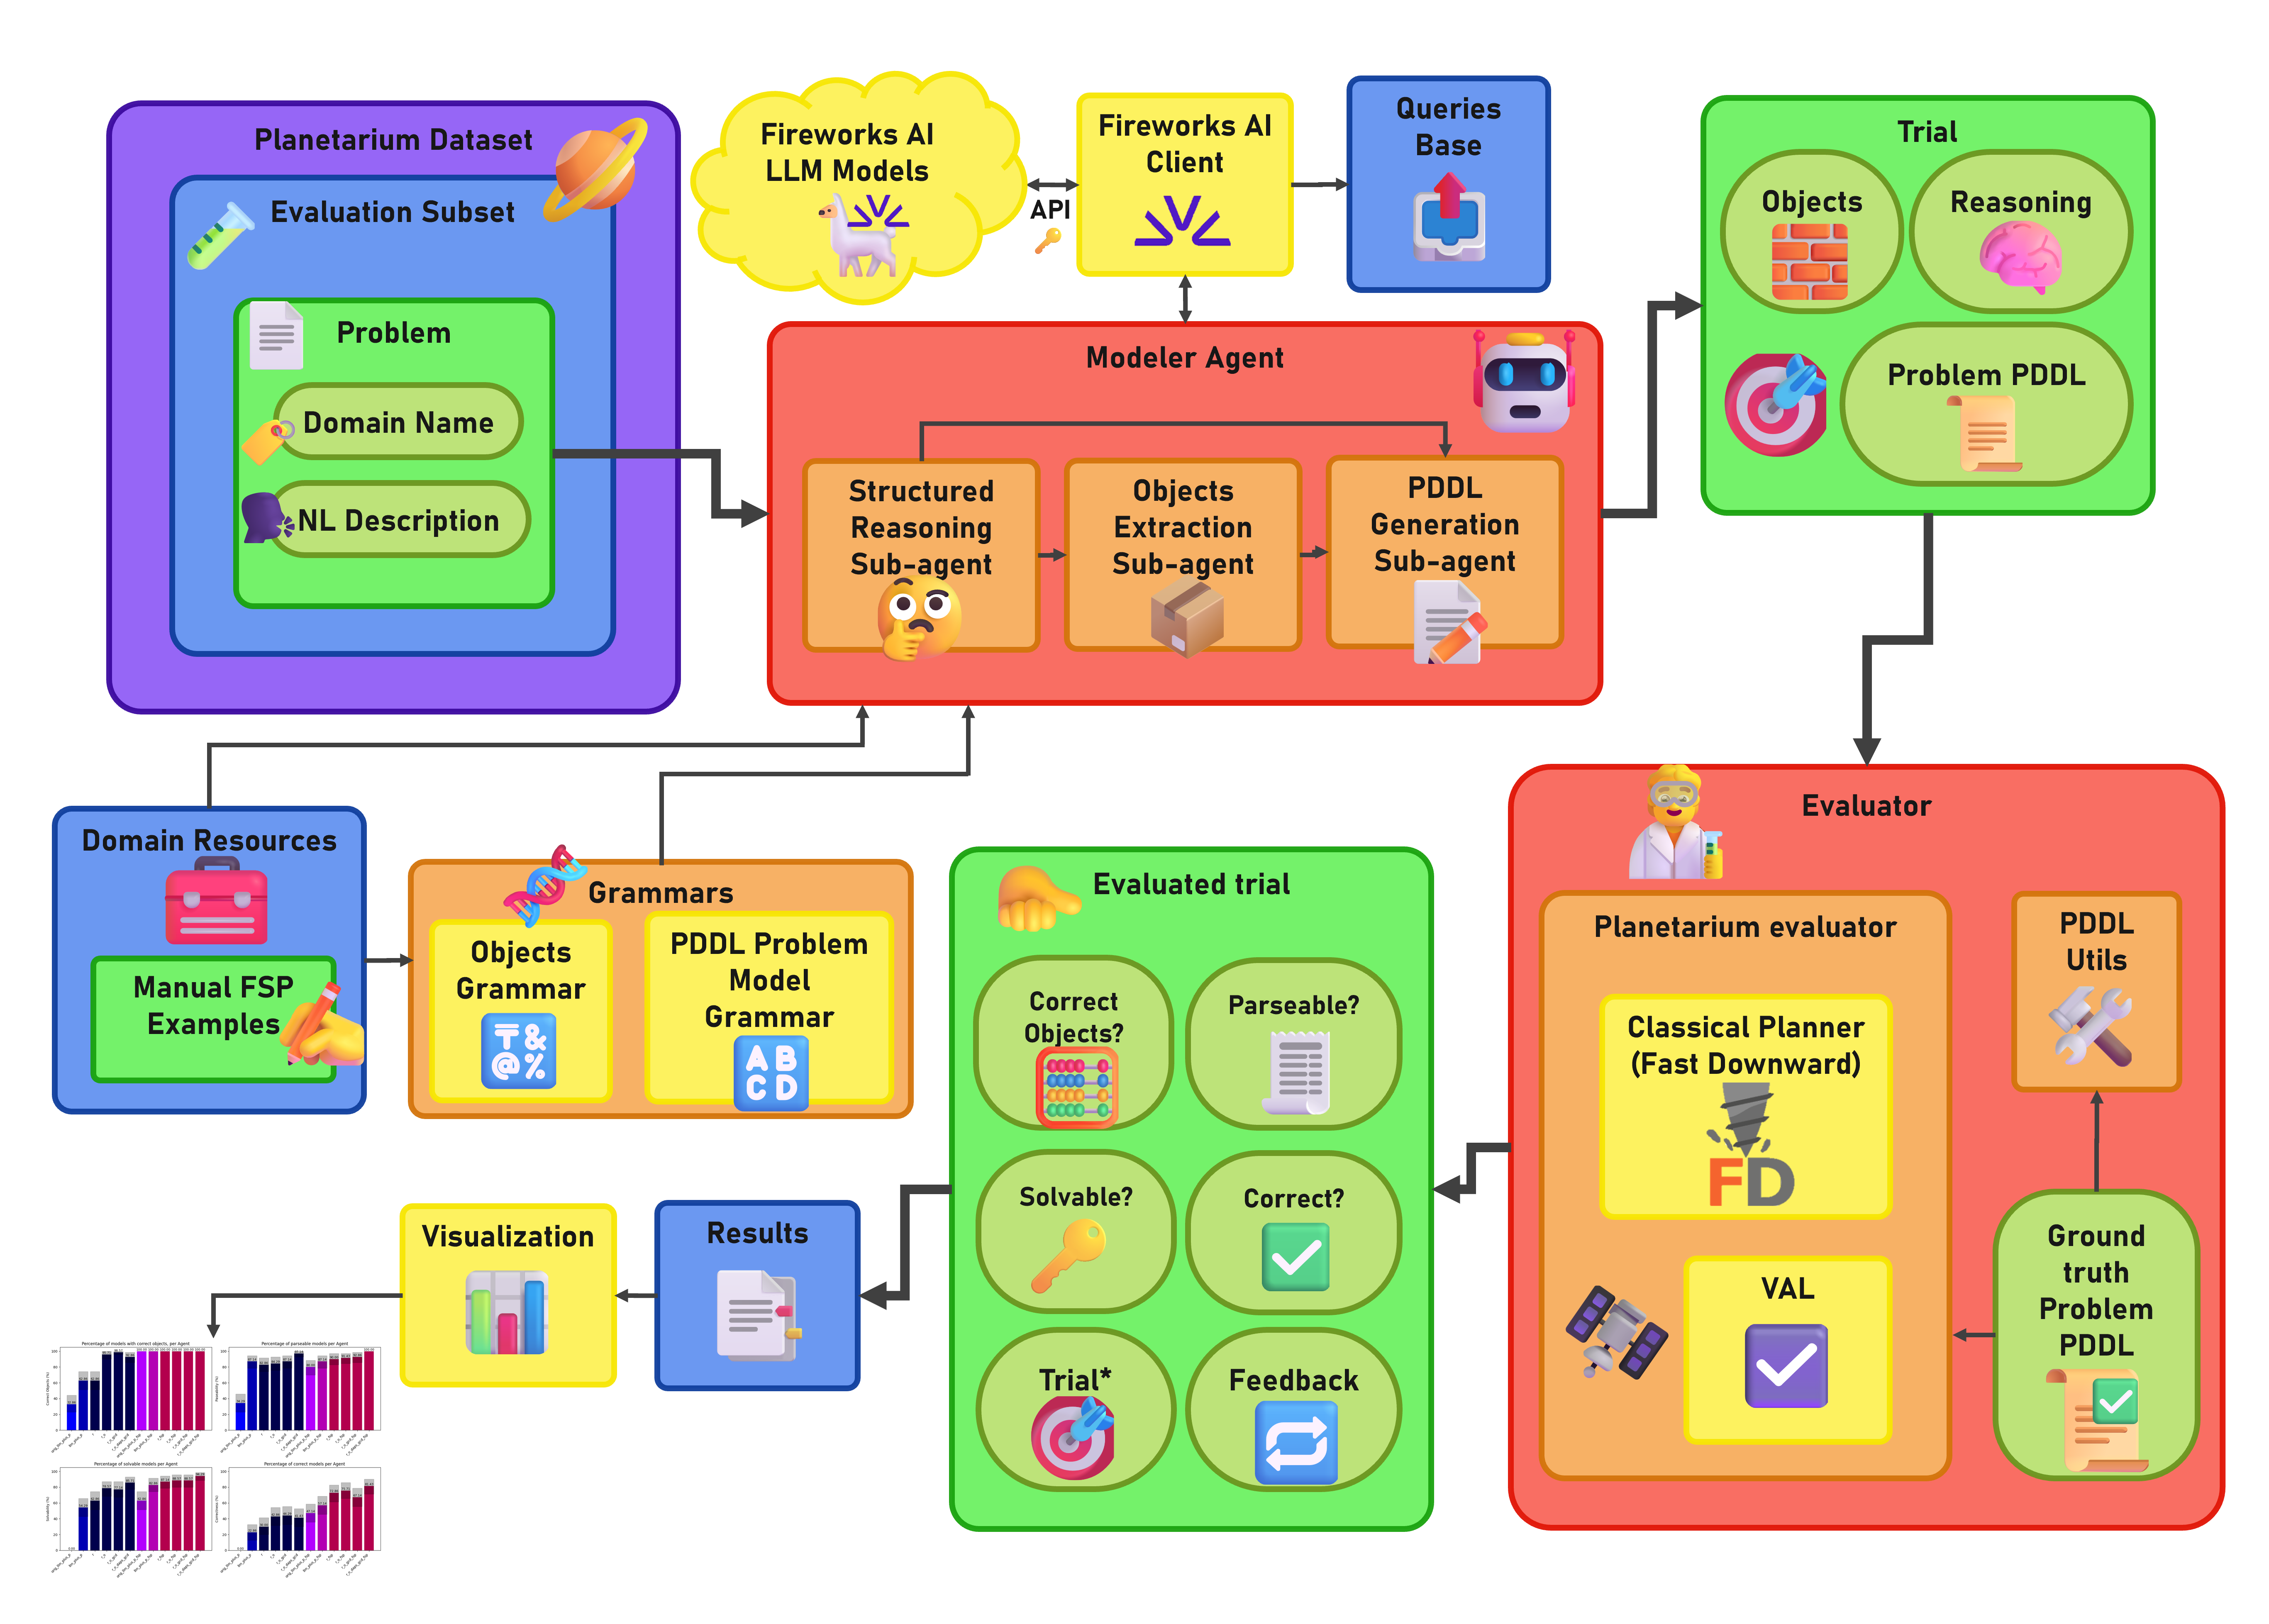
\includegraphics[width=0.9\textwidth]{Graphics/evaluation.png}
\caption{Flujo de evaluación de los agentes modeladores propuestos.}
\label{fig:objects}
\end{figure}

\section{\textit{Baselines}}

Con el fin de evaluar el impacto de los métodos propuestos para mejorar la generación de modelos \textit{PDDL}, se realiza una comparación con los agentes presentados en el trabajo \textit{LLM+P} \parencite{liu2023llm+}. Este trabajo incluye tanto un agente planificador como un agente modelador, ambos en modalidad \textit{Zero-Shot} (sin ejemplos previos), así como sus respectivas variantes \textit{One-Shot} (con un ejemplo fijo).

Se concibe una reproducción fiel de los agentes modeladores originales, realizando únicamente adaptaciones necesarias en sus \textit{prompts} para adecuarlos a los dominios del \textit{benchmark} \textit{Planetarium}. Si bien el dominio \textit{Blocksworld} coincide exactamente con el utilizado en \textit{LLM+P}, los dominios \textit{Gripper} y \textit{Floor-Tile} presentan pequeñas diferencias estructurales. Por esta razón, se adaptaron los ejemplos de \textit{FSP} manteniendo la intención de los problemas originales, pero reformulados según las variantes correspondientes de \textit{Planetarium}.

Se observó que los \textit{prompts} utilizados en el trabajo original eran considerablemente subóptimos para una evaluación automatizada en el entorno de \textit{Planetarium}, particularmente en el caso \textit{Zero-Shot}. En esta modalidad, el único contexto proporcionado al agente modelador es la descripción en lenguaje natural de las acciones disponibles. A partir de esta descripción, el agente debe inferir la totalidad de los predicados requeridos por el modelo \textit{PDDL}, incluyendo su nombre y sus argumentos. Esta condición genera una desventaja significativa, ya que la evaluación automática de \textit{Planetarium} exige que los predicados utilizados coincidan exactamente con aquellos definidos en el dominio.

En el trabajo original, este tipo de desalineaciones no representaba una limitación crítica debido a que la evaluación de los modelos \textit{PDDL} generados se realizaba manualmente. Por el contrario, en el presente trabajo se requiere una validación automática que depende estrictamente de la precisión sintáctica y semántica de los modelos generados.

En la modalidad \textit{One-Shot}, el agente recibe como entrada un ejemplo completo, pero sin la descripción explícita de todos los predicados disponibles. Aunque este enfoque ofrece al agente más información que la modalidad \textit{Zero-Shot}, todavía presenta deficiencias importantes en cobertura y comprensión semántica.

Por estas razones, se propone una reimplementación de los agentes modeladores originales, incorporando el modelo \textit{PDDL} del dominio como parte del contexto, además de una estructura de \textit{prompt} mejorada. A partir de estas versiones se pretende derivar los agentes propuestos en esta tesis, a los cuales se integran los distintos módulos de mejora.

De igual forma, los agentes planificadores son reimplementados, realizando ligeros ajustes en los \textit{prompts} con el objetivo de presentar explícitamente el formato de las acciones disponibles y adecuarlos a las particularidades de las variantes de \textit{Planetarium}.

\subsection{Agentes planificadores}

Los agentes planificadores propuestos utilizan \textit{LLMs} para resolver tareas de planificación automática. A partir de la entrada compuesta por el modelo del dominio en \textit{PDDL} y la descripción en lenguaje natural del problema, generan como salida un plan válido en el formato requerido por el validador externo \textit{VAL}, así como el conteo de \textit{tokens} consumidos durante la generación.

Basados en el enfoque propuesto en \textit{LLM+P}, se proponen dos variantes de agentes cuya única diferencia es la inclusión opcional de un ejemplo de tipo \textit{FSP} en el \textit{prompt}. Esta inclusión es modular y depende de los objetivos del experimento. Ambos agentes comparten una misma plantilla general que estructura la información presentada al modelo.

El \textit{prompt} comienza situando al modelo en el rol de un agente de planificación avanzado. Luego se introduce el dominio: su nombre, una breve descripción en lenguaje natural y el listado de acciones disponibles. Esta información proviene de una base de recursos estructurada por dominio, construida a partir de conocimiento experto. A continuación, se describe la tarea a realizar y se especifica el formato de salida esperado, también obtenido automáticamente desde la misma base.

Cuando se activa el módulo \textit{FSP}, se incorpora un ejemplo representativo del dominio, compuesto por una descripción del problema y su plan correspondiente. Este ejemplo sirve como guía contextual y es tomado directamente del conjunto de recursos por dominio.

Finalmente, se presenta el nuevo problema a resolver, tal como aparece en el \textit{dataset} de \textit{Planetarium}, y se espera que el modelo complete la sección final con el plan correspondiente.

\subsection{Agentes modeladores originales}

Los agentes modeladores originales, inspirados en la propuesta de \textit{LLM+P} \parencite{liu2023llm+}, generan como salida un archivo \textit{PDDL} que representa formalmente el problema de planificación descrito en lenguaje natural. Además, se incorpora como métrica auxiliar el número total de \textit{tokens} utilizados durante la generación, para facilitar el análisis de eficiencia.

La definición y \textit{prompt} de estos agentes varía en función de si se encuentra o no activado el módulo \textit{FSP}, que determina la presencia de ejemplos explícitos en el \textit{prompt}. Cuando dicho módulo no está activo, el modelo recibe como contexto una descripción del dominio —incluyendo sus acciones disponibles— seguida directamente por el problema en lenguaje natural a resolver. Toda esta información es obtenida desde la base de recursos por dominio, construida a partir de conocimiento experto. El modelo debe entonces generar el archivo \textit{PDDL} correspondiente, sin explicaciones intermedias.

En la modalidad con \textit{FSP}, el agente recibe primero un ejemplo completo, que incluye la descripción en lenguaje natural de un problema representativo y su respectivo archivo \textit{PDDL}. A continuación, se presenta un nuevo problema cuya descripción debe ser transformada, nuevamente, en su representación formal. Los ejemplos utilizados en esta variante fueron elaborados manualmente y adaptados desde la propuesta original de \textit{LLM+P}, ajustándolos a las especificidades de los dominios del \textit{benchmark Planetarium}.

Este diseño modular del \textit{prompt} permite estudiar el impacto de la demostración explícita de pares problema-solución sobre la calidad del modelado automático.

\section{Agentes modeladores propuestos}

La solución propuesta consiste en un agente generador de modelos \textit{PDDL}, diseñado para ser modular y extensible. A partir de una versión mejorada de los agentes modeladores originales —descritos en la sección anterior— se construye una base común utilizada tanto en los \textit{baselines} reforzados como en las variantes experimentales con módulos avanzados. Esta arquitectura permite incorporar, de manera controlada, múltiples mecanismos de mejora.

El agente base recibe como entrada el identificador numérico del problema, el dominio correspondiente y su descripción en lenguaje natural. Como salida, produce el archivo \textit{PDDL} que modela el problema y el conteo total de \textit{tokens} consumidos en la generación.

Con el objetivo de facilitar la comparación entre variantes, se adopta una estructura de \textit{prompt} estandarizada, sobre la cual se añaden condicionalmente diferentes bloques. El \textit{prompt} comienza estableciendo que el modelo actúa como un agente especializado en generación de \textit{PDDL}, y presenta al LLM el nombre y una breve descripción del dominio, junto con su definición formal en \textit{PDDL}\footnote{En el caso del dominio \textit{Floor-Tile}, con inclusión de ejemplo \textit{FSP}, se opta por omitir las acciones definidas en el \textit{PDDL} del dominio provisto, pues se observó mejor rendimiento que al agregarlos tanto en el \textit{prompt} de generación de \textit{PDDL} como en el de extracción de objetos. Esto se puede deber a que estas acciones no proveen de conocimiento relevante para esas fases, sino que representan ruido innecesario. En la fase de razonamiento, sin embargo, sí contribuye positivamente al rendimiento.}. A continuación, se enuncia la tarea: generar un modelo de problema en \textit{PDDL} que se ajuste a los requerimientos del subconjunto correspondiente, específicamente \textit{:strips} o \textit{:strips + :typing}, según la presencia o no de tipos. Estos componentes se extraen de la base de recursos de dominio instanciada por el experto.

De forma opcional, se puede incluir una indicación sobre el uso de comentarios en la sección \textit{:init} o \textit{:goal}, cuando el módulo \textit{Comments} está activado. También puede incorporarse una o más demostraciones mediante ejemplos completos (\textit{Few-Shot Prompting}, módulo \textit{FSP}), seleccionados de forma manual desde la base de recursos del dominio, o recuperados dinámicamente por un componente \textit{Retriever} en caso de la activación del módulo de \textit{RAG}.

Cada ejemplo presenta la descripción en lenguaje natural del problema, razonamientos previos y objetos relevantes si están activos los módulos \textit{Reasoning} y \textit{Objects Extraction}, respectivamente, seguidos del modelo \textit{PDDL} correspondiente.

Cuando el módulo \textit{Insights} está habilitado, el \textit{prompt} incluye un conjunto estructurado de conocimientos adquiridos previamente, organizados en tres categorías: conocimiento del mundo del dominio, y reglas o buenas prácticas de modelado de planificación, generales y específicas del dominio. Este conocimiento busca guiar al modelo, basado en experiencia acumulada.

En la parte final del \textit{prompt} se presenta el nuevo problema a resolver, expresado en lenguaje natural. Si el agente pertenece al subconjunto experiencial, y no es el primer intento sobre ese problema, se añade un bloque de reflexión que incluye la salida previa generada, el \textit{feedback} de evaluación automática, y una reflexión explícita generada por un sub-agente. Esta capacidad permite reintentos con autocrítica fundamentada, constituyendo un ciclo de mejora iterativa.

Finalmente, en presencia de los módulos de razonamiento y extracción de objetos, el \textit{prompt} puede incorporar razonamientos sobre el problema, así como la lista de objetos que deberían ser utilizados, ambos generados por sub-agentes especializados en una fase previa. Estos componentes se explican a detalle en la sección siguiente. Esta integración progresiva y jerárquica de información permite una evaluación sistemática del impacto de cada técnica sobre la calidad del modelado, respetando siempre la estructura común del \textit{prompt} para garantizar la comparabilidad entre configuraciones.

Los algoritmos de instanciación del agente modelador, su asignación de un nuevo problema a modelar, y su proceso de resolución se presentan a modo de pseudocódigos en los Anexos.

\subsection{Razonamiento}

Diversos trabajos previos han demostrado que permitir a los \textit{LLM} realizar razonamientos previos a la ejecución de una tarea puede mejorar significativamente la calidad de sus resultados. Siguiendo esta línea de investigación, se propone una fase de razonamiento, previa y separada de la generación del modelo \textit{PDDL}. Esta separación se realiza con el objetivo de modularizar el proceso, facilitar la inspección individual del razonamiento generado y permitir su reutilización en diferentes fases de modelado del problema. Además, el razonamiento explícito constituye una fuente valiosa de explicabilidad del proceso de generación automática, alineándose con principios de transparencia y trazabilidad.

El razonamiento se lleva a cabo por medio de un \textit{prompt} distinto, diseñado para inducir al \textit{LLM} a adoptar el rol de un agente especializado en análisis y razonamiento sobre la modelación de tareas de planificación. El \textit{prompt} guía de forma estructurada al modelo para razonar en tres fases bien delimitadas: \textbf{objetos}, \textbf{estado inicial} y \textbf{estado objetivo}. Estas fases reflejan directamente la estructura del modelo \textit{PDDL} de problema que se generará posteriormente, permitiendo que el razonamiento funcione como un soporte semántico directo para la construcción del modelo.

\begin{itemize}
    \item En la sección de \textbf{objetos}, se requiere enumerar de forma explícita todos los objetos mencionados o inferidos a partir de la descripción del problema. Estos objetos se corresponden con los elementos declarados en la sección \texttt{:objects} del modelo \textit{PDDL}.

    \item En la sección de \textbf{estado inicial}, el modelo debe describir detalladamente la situación inicial del problema. Se permite que el agente haga suposiciones razonables en caso de que la descripción del problema provea información ambigua o incompleta. Este contenido se traduce posteriormente en los predicados de la sección \texttt{:init}.

    \item Finalmente, en la sección de \textbf{estado objetivo}, se indica el conjunto de condiciones que deben cumplirse para considerar que el problema ha sido resuelto. Nuevamente, se induce razonamiento para completar posibles lagunas semánticas. Esta parte se traduce en la sección \texttt{:goal} del modelo \textit{PDDL}.
\end{itemize}

El \textit{prompt} utilizado establece el rol del modelo como un agente experto en razonamiento aplicado a planificación, y presenta el dominio con su descripción en lenguaje natural, su definición formal en \textit{PDDL} y una descripción textual del nuevo problema. Se solicita razonar paso a paso para resolver ambigüedades y anticipar la construcción del modelo \textit{PDDL}, mediante tres párrafos concisos con la intención anteriormente descrita. Se permite la inferencia explícita en caso de información incompleta, y se enfatiza que no debe razonarse sobre la planificación en sí, sino únicamente sobre la representación del problema. De manera análoga al \textit{prompt} principal, pueden añadirse ejemplos previos (\textit{FSP}), \textit{insights}, o reflexiones de intentos anteriores, dependiendo de los módulos activos.

\subsection{Extracción de Objetos}

Con el objetivo de anclar de forma más precisa la generación del modelo \textit{PDDL}, se propone una fase adicional de extracción estructurada de los objetos que participan en el problema de planificación. Esta fase no solo permite listar de forma clara y detallada los objetos que forman parte de los predicados en las secciones \texttt{:init} y \texttt{:goal}, sino que también facilita la construcción de una gramática más restrictiva para el \textit{GCD}. La salida del modelo en esta fase también es restringida mediante una gramática especializada. Ambas se explican a detalle en la siguiente sección.

La extracción de objetos se realiza como una etapa independiente y posterior a la fase de razonamiento (cuando esta se encuentra activa), permitiendo aprovechar directamente la información inferida en dicha fase y garantizar la consistencia entre ambos procesos. Los objetos extraídos, así como sus posibles tipos, son representados en formato \textit{JSON}, de forma estructurada y con el nivel de detalle necesario para apoyar tanto la generación posterior del \textit{PDDL} como el uso de técnicas que dependen del conocimiento explícito de la estructura del problema.

El \textit{prompt} empleado define al modelo como un agente especializado en extracción de objetos, y presenta el dominio con su descripción en lenguaje natural y su definición formal en \textit{PDDL}. Luego, se introduce el problema a resolver, y se solicita generar una lista completa de objetos relevantes en formato \textit{JSON}. Si el dominio es tipado, se indica que los objetos deben agruparse por tipo. Además, dependiendo de los módulos activos, el \textit{prompt} puede incluir ejemplos previos (\textit{FSP}), razonamiento generado previamente, o información proveniente de intentos fallidos anteriores. En particular, la reflexión sobre fallos se incluye solo si no está activa la fase de razonamiento, ya que agregar el resultado de ambas sería redundante.

\section{\textit{Grammar-Constrained Decoding (GCD)}}

Con el objetivo de asegurar la correctitud sintáctica de los modelos \textit{PDDL} generados, se propone el uso de la técnica de \textit{GCD}. Esta técnica permite imponer una gramática libre de contexto a la salida generada por un modelo de lenguaje, garantizando que la estructura del texto producido respete determinadas reglas sintácticas.

Los modelos de \textit{Fireworks AI}, utilizados en este trabajo, soportan de forma nativa la inclusión de gramáticas \textit{GBNF} a través de su \textit{API}. En el presente trabajo, la técnica de \textit{GCD} es empleada para dos propósitos fundamentales: la generación de modelos \textit{PDDL} de problema y la extracción estructurada de objetos, descrita previamente.

\subsection{\textit{GCD} para generación de modelos \textit{PDDL} de problema}

El primer paso consiste en construir una gramática general en formato \textit{GBNF} que cubra el subconjunto de \texttt{:strips + :typing} del lenguaje \textit{PDDL} para modelos de problema. Para ello, se parte de la definición original en \textit{BNF} de \textit{PDDL 3.1} \parencite{kovacs2011bnf}, la cual es filtrada y adaptada cuidadosamente para ajustarse tanto al subconjunto requerido como al formato \textit{GBNF} exigido por el sistema.

Durante este proceso se definen varios niveles de especificidad en la aplicación de la gramática:

\begin{itemize}
    \item \textbf{Base:} se define una gramática general válida para todo dominio que utilice el subconjunto \texttt{:strips + :typing}.
    \item \textbf{Restricción por dominio:} se limita el conjunto de predicados permitidos en las secciones \texttt{:init} y \texttt{:goal} a los definidos por el dominio correspondiente.
    \item \textbf{Restricción por aridad:} se asegura que la aridad de los predicados utilizados coincida exactamente con la declarada en el dominio.
    \item \textbf{Restricción por objetos:} se restringen los objetos utilizados a los declarados explícitamente en la sección \texttt{:objects} y, en dominios tipados, se verifica además que los tipos asignados a los argumentos de los predicados coincidan con los tipos de los objetos correspondientes.
\end{itemize}

El nivel de especificidad de la gramática generada depende de los módulos activos en el agente modelador. Se definen dos módulos relevantes: \textit{GCD} y \textit{DAPS} (acrónimo de \textit{Domain-and Problem-Specific}, es decir, ``específico del dominio y del problema''). Cuando el módulo \textit{GCD} está activo, la generación se realiza utilizando una gramática restringida. Si además está activo el módulo \textit{DAPS}, se incluyen las restricciones más específicas relacionadas con los predicados y/u objetos particulares del problema dado.

La estructura general de la gramática \textit{GBNF} es la siguiente:

\begin{tcolorbox}[colback=blue!5!white, colframe=blue!75!black, title=Gramática \textit{GBNF} general, fonttitle=\bfseries, breakable]
\small
\begin{verbatim}
root ::= define
define ::= "(" ws "define" ws problemDecl domainDecl requireDef 
            objectDecl init goal ")"

problemDecl ::= "(" ws "problem" ws "<Nombre del problema>" ws ")" ws
domainDecl ::= "(" ws ":domain" ws "<Nombre del dominio>" ws ")" ws
objectDecl ::= "(" ws ":objects" ws <Objetos> ws ")" ws
requireDef ::= "(" ws ":requirements" ws "<Requerimientos>" ws ")" ws
init ::= "(" ws ":init" ws initEl* ")" ws
initEl ::= literal
goal ::= "(" ws ":goal" ws preGD ")" ws

<Producción de literal>
<Producción de fórmula atómica>

preGD ::= "(and" ws GD+ ")"
<Producción de GD>

<Producciones de los objetos>
ws ::= [ \t\n]*
\end{verbatim}
\end{tcolorbox}

Los elementos entre signos \texttt{<...>} representan fragmentos variables que dependen del problema de planificación, del dominio y de los módulos activos:

\begin{itemize}
    \item \texttt{<Nombre del problema>} y \texttt{<Nombre del dominio>} se determinan a partir del problema específico que se desea modelar.
    \item \texttt{<Requerimientos>} toma el valor \texttt{:strips :typing} si el dominio está tipado, y \texttt{:strips} en caso contrario.
    \item \texttt{<Producción de literal>} y \texttt{<Producción de GD>} varían según la inclusión del módulo \textit{Comments}, que permite añadir comentarios en el modelo \textit{PDDL}. 
\end{itemize}

Si el módulo \textit{Comments} no está activo, las producciones son:

\begin{tcolorbox}[colback=blue!5!white, colframe=blue!75!black, title=Producciones sin módulo \textit{Comments}, fonttitle=\bfseries, breakable]
\small
\begin{verbatim}
literal ::= atomicFormula ws
GD ::= atomicFormula ws
\end{verbatim}
\end{tcolorbox}

En caso contrario, se añade la posibilidad de insertar comentarios al inicio de cada predicado:

\begin{tcolorbox}[colback=blue!5!white, colframe=blue!75!black, title=Producciones con módulo \textit{Comments}, fonttitle=\bfseries, breakable]
\small
\begin{verbatim}
literal ::= comment atomicFormula ws | atomicFormula ws
GD ::= comment atomicFormula ws | atomicFormula ws
comment ::= ";" [^\n]* "\n"
\end{verbatim}
\end{tcolorbox}

\subsection{Componentes específicos según inclusión del módulo \textit{DAPS}}

Los componentes variables de la gramática \textit{GBNF} ---específicamente \texttt{<Objetos>}, \texttt{<Producciones de los objetos>} y \texttt{<Producción de fórmula atómica>}--- dependen directamente de la activación o no del módulo \textit{DAPS}. A continuación se describen detalladamente ambos escenarios.

\subsubsection{Sin inclusión del módulo \textit{DAPS}}

Cuando el módulo \textit{DAPS} no está activo, la gramática permite una mayor libertad en la generación del modelo \textit{PDDL}, admitiendo cualquier nombre para objetos y tipos. Los fragmentos relevantes son los siguientes:

\begin{tcolorbox}[colback=blue!5!white, colframe=blue!75!black, title=Fragmento \texttt{<Objetos>} sin \textit{DAPS}, fonttitle=\bfseries, breakable]
\small
\begin{verbatim}
typedList
\end{verbatim}
\end{tcolorbox}

\begin{tcolorbox}[colback=blue!5!white, colframe=blue!75!black, title=Producciones de los objetos sin \textit{DAPS}, fonttitle=\bfseries, breakable]
\small
\begin{verbatim}
typedList ::= <typedList RHS>
type ::= "(either" primitiveType+ ")" | primitiveType
primitiveType ::= name | "object"

name ::= letter anyChar*
letter ::= [a-zA-Z]
anyChar ::= letter | digit | "-" | "_"

digit ::= [0-9]
\end{verbatim}
\end{tcolorbox}

El componente \texttt{<typedList RHS>} (\textit{Right-Hand Side - RHS}) depende de si el dominio es tipado:
\begin{itemize}
    \item En dominios tipados: \texttt{(name ws)+ "-" ws type ws)+}
    \item En dominios no tipados: \texttt{(name ws)*}
\end{itemize}

Finalmente, la producción de fórmulas atómicas también es completamente general:

\begin{tcolorbox}[colback=blue!5!white, colframe=blue!75!black, title=Producción de fórmula atómica sin \textit{DAPS}, fonttitle=\bfseries, breakable]
\small
\begin{verbatim}
atomicFormula ::= "(" name (ws object)* ")"
\end{verbatim}
\end{tcolorbox}

Esta formulación no impone restricciones sobre el conjunto de predicados permitidos, ni sobre su aridad o los tipos de argumentos, por lo que es más propensa a errores semánticos, aunque garantiza la sintaxis básica.

\subsubsection{Con inclusión del módulo \textit{DAPS}}

La activación del módulo \textit{DAPS} permite restringir fuertemente la generación, ajustándola al dominio y problema específicos. Para ello, se utilizan tanto los predicados definidos en el dominio, incluyendo su aridad (o tipos de argumentos en caso de dominios tipados), como los objetos obtenidos durante la fase de extracción estructurada.

\paragraph{Dominios no tipados}

En estos casos, \texttt{<Objetos>} se representa como una lista de nombres separados por espacio, entre comillas dobles. Por ejemplo, si los objetos extraídos de un problema de \textit{Blocksworld} son \texttt{[b1, b2, b3]} el fragmento queda:

\begin{tcolorbox}[colback=white, colframe=gray, title=Ejemplo de fragmento \texttt{<Objetos>} no tipado con \textit{DAPS}, fonttitle=\bfseries, breakable]
\small
\begin{verbatim}
"b1 b2 b3"
\end{verbatim}
\end{tcolorbox}

\texttt{<Producciones de los objetos>} se sustituye por: 
\begin{tcolorbox}[colback=blue!5!white, colframe=blue!75!black, title=Fragmento \texttt{<Objetos>} no tipado con \textit{DAPS}, fonttitle=\bfseries, breakable]
\small
\begin{verbatim}
object ::= "<obj1>" | "<obj2>" | ... | "<objn>"
\end{verbatim}
\end{tcolorbox}

Donde \texttt{<obj1>, <obj2>, ..., <objn>} son los nombres de los objetos determinados en la fase de extracción, cada uno entre comillas dobles y todos unidos mediante el operador de disyunción \texttt{|}. La producción correspondiente al ejemplo anterior restringe de forma explícita los objetos disponibles:

\begin{tcolorbox}[colback=white, colframe=gray, title=Ejemplo de producciones de los objetos no tipados con \textit{DAPS}, fonttitle=\bfseries, breakable]
\small
\begin{verbatim}
object ::= "b1" | "b2" | "b3"
\end{verbatim}
\end{tcolorbox}

\texttt{<Producción de fórmula atómica>} considera cada predicado posible y su aridad exacta.  En este caso empieza con el prefijo \texttt{atomicFormula ::=}, y por cada predicado proporcionado del dominio se construyen las opciones posibles de fórmulas atómicas, unidas por el operador de disyunción \texttt{|}. Cada opción es de la forma:
\begin{tcolorbox}[colback=blue!5!white, colframe=blue!75!black, title=Producción de fórmula atómica en dominios no tipados con \textit{DAPS}, fonttitle=\bfseries, breakable]
\small
\begin{verbatim}
"(<Nombre del predicado>"
 (ws object){<Aridad del predicado>} ")"
\end{verbatim}
\end{tcolorbox}

Donde \texttt{<Nombre del predicado>} y \texttt{<Aridad del predicado>} se sustituyen por sus valores correspondientes. Por ejemplo, para el predicado \texttt{(on ?x ?y)} del dominio \textit{Blocksworld}, se construye el siguiente fragmento:

\begin{tcolorbox}[colback=white, colframe=gray, title=Ejemplo de producción de fórmula atómica con \textit{DAPS} (no tipado), fonttitle=\bfseries, breakable]
\small
\begin{verbatim}
atomicFormula ::= "(on" ws (object){2} ")"
\end{verbatim}
\end{tcolorbox}


\paragraph{Dominios tipados}

En dominios que incluyen tipado, \texttt{<Objetos>} se organiza por tipo, de la forma:

\begin{tcolorbox}[colback=blue!5!white, colframe=blue!75!black, title=Objetos en dominios tipados con \textit{DAPS}, fonttitle=\bfseries, breakable]
\small
\begin{verbatim}
"<Objetos de tipo 1> <Objetos de tipo 2> ... <Objetos de tipo m>"
\end{verbatim}
\end{tcolorbox}

Donde cada fragmento \texttt{<Objetos de tipo i>} es una lista con los nombres de los objetos de dicho tipo, y terminada con el sufijo \texttt{- <Nombre del tipo>}. Por ejemplo, en  \textit{Floor-Tile}, sean los objetos extraídos:

\begin{tcolorbox}[colback=white, colframe=gray, title=Ejemplo de \texttt{<Objetos>} en dominios tipados con \textit{DAPS}, fonttitle=\bfseries, breakable]
\small
\begin{verbatim}
{
	"tile": ["tile1", "tile2", "tile3", "tile4"],
	"robot": ["robot1", "robot2"],
	"color": ["color1"]
}
\end{verbatim}
\end{tcolorbox}

El fragmento queda:

\begin{tcolorbox}[colback=white, colframe=gray, title=Fragmento \texttt{<Objetos>} en dominios tipados con \textit{DAPS}, fonttitle=\bfseries, breakable]
\small
\begin{verbatim}
"tile1 tile2 tile3 tile4 - tile robot1 robot2 - robot color1 - color"
\end{verbatim}
\end{tcolorbox}

Las producciones de objetos y de fórmulas atómicas se restringen, además, en función de los tipos esperados por los predicados.

Esto permite al modelo generar únicamente estructuras válidas desde el punto de vista sintáctico y semántico, respetando tanto los tipos como las aridades esperadas.

\texttt{<Producciones de los objetos>} es un conjunto de producciones (una por cada tipo del dominio) separadas por líneas de la forma:
\begin{tcolorbox}[colback=blue!5!white, colframe=blue!75!black, title=Producciones de los objetos por tipo (tipado con \textit{DAPS}), fonttitle=\bfseries, breakable]
\small
\begin{verbatim}
obj-<Nombre del tipo> ::= "<obj1>" | "<obj2>" | ... | "<objn>"
\end{verbatim}
\end{tcolorbox}

Donde \texttt{<obj1>, <obj2>, ..., <objn>} son los nombres de los objetos extraídos cuya clasificación corresponde a ese tipo o a alguno de sus subtipos. Siguiendo el ejemplo anterior, el fragmento resultante sería:

\begin{tcolorbox}[colback=white, colframe=gray, title=Ejemplo de producciones por tipo, fonttitle=\bfseries, breakable]
\small
\begin{verbatim}
obj-tile ::= "tile1" | "tile2" | "tile3" | "tile4"
obj-robot ::= "robot1" | "robot2"
obj-color ::= "color1"
\end{verbatim}
\end{tcolorbox}

Estas producciones asumen que cada objeto pertenece a exactamente un tipo. Asimismo, se asume una jerarquía de tipos sin multiherencia, lo cual es una simplificación válida dado que, aunque el lenguaje \textit{PDDL} permite multiherencia, la gran mayoría de dominios utilizados en \textit{benchmarks} estándar como \textit{IPC} no la emplean. Esta suposición permite construir un árbol de herencia de tipos con \texttt{object} como raíz.

Formalmente, si se tiene un conjunto de tipos \( T \) y una relación de herencia \( \prec \subseteq T \times T \), donde \( t_1 \prec t_2 \) indica que \( t_1 \) es subtipo de \( t_2 \), entonces el conjunto de objetos incluidos en la producción \texttt{obj-\textit{t}} es:

\[
\mathcal{O}_t = \{ o \in O \mid type(o) = t' \text{ y } t' \sqsubseteq t \}
\]

donde \( \sqsubseteq \) es la clausura reflexiva y transitiva de \( \prec \), y \( type(o) \) es el tipo de \( o \).

\vspace{1em}
La \texttt{<Producción de fórmula atómica>} también se adapta para aprovechar esta estructura. Se inicia con el prefijo:

\begin{tcolorbox}[colback=blue!5!white, colframe=blue!75!black, title=Estructura general de \texttt{atomicFormula}, fonttitle=\bfseries, breakable]
\small
\begin{verbatim}
atomicFormula ::= 
\end{verbatim}
\end{tcolorbox}

y por cada predicado definido en el dominio, se añade una opción con su nombre y las producciones de objetos correspondientes a los tipos de sus argumentos. Cada opción toma la forma:

\begin{tcolorbox}[colback=blue!5!white, colframe=blue!75!black, title=Plantilla por predicado (tipado), fonttitle=\bfseries, breakable]
\small
\begin{verbatim}
"(<Nombre del predicado>" ws obj-<Tipo1> ws ... ws obj-<Tipok> ws ")"
\end{verbatim}
\end{tcolorbox}

Por ejemplo, para el predicado \texttt{(robot-at ?r - robot ?x - tile)}, la producción correspondiente sería:

\begin{tcolorbox}[colback=white, colframe=gray, title=Ejemplo \texttt{atomicFormula} para predicado tipado, fonttitle=\bfseries, breakable]
\small
\begin{verbatim}
"(robot-at" ws obj-robot ws obj-tile ws ")"
\end{verbatim}
\end{tcolorbox}

Esto permite una validación estricta no solo sintáctica, sino también semántica, al restringir los objetos posibles según su tipo esperado.

\subsection{\textit{GCD} para extracción de objetos en dominios no tipados}

Para asegurar la validez sintáctica en la fase de extracción estructurada de objetos cuando el dominio no es tipado, se construye también una gramática \textit{GBNF} dedicada a esta tarea. La gramática es diseñada para aceptar exclusivamente cadenas que representaran una estructura tipo \textit{JSON} con una sola clave llamada \texttt{objects}, cuyo valor es una lista de cadenas que representaran los nombres de los objetos:

\begin{tcolorbox}[colback=blue!5!white, colframe=blue!75!black, title=Gramática para extracción de objetos (no tipado), fonttitle=\bfseries, breakable]
\small
\begin{verbatim}
root ::= "{" dq "objects" dq ": [" obj (", " obj)* "]" "}"
obj ::= dq letter anyChar* dq

letter ::= [a-zA-Z]
anyChar ::= letter | digit | "-" | "_"
digit ::= [0-9]
dq ::= "\\\""
\end{verbatim}
\end{tcolorbox}

Este esquema asegura una estructura válida en la respuesta del modelo, acorde con el formato esperado por los módulos posteriores. Por ejemplo, en un problema del dominio \textit{Blocksworld} que involucra los bloques \texttt{b1}, \texttt{b2}, \texttt{b3} y \texttt{b4}, la salida generada por el agente tiene la forma:

\begin{tcolorbox}[colback=white, colframe=gray, title=Ejemplo de salida válida (no tipado), fonttitle=\bfseries, breakable]
\small
\begin{verbatim}
{"objects": ["b1", "b2", "b3", "b4"]}
\end{verbatim}
\end{tcolorbox}

De esta manera, la aplicación de \textit{GCD} a esta fase también garantiza una representación formalmente consistente de los objetos extraídos, lo que resulta clave para los pasos posteriores en la construcción del problema en \textit{PDDL}.

\subsection{\textit{GCD} para extracción de objetos en dominios tipados}

Cuando el dominio de planificación es tipado, se utiliza una gramática específica para la fase de extracción de objetos. Esta gramática permite representar una estructura tipo \textit{JSON} en la que cada tipo del dominio se asocia con una lista de objetos del problema actual. La gramática general propuesta es la siguiente:

\begin{tcolorbox}[colback=blue!5!white, colframe=blue!75!black, title=Gramática para extracción de objetos (dominios tipados), fonttitle=\bfseries, breakable]
\small
\begin{verbatim}
root ::= <Descripción del diccionario de objetos>
obj-list ::= "[" obj (", " obj)* "]"
obj ::= dq letter anyChar* dq

letter ::= [a-zA-Z]
anyChar ::= letter | digit | "-" | "_"
digit ::= [0-9]

tab ::= "\t"
dq ::= "\\\""
el ::= "\n"
\end{verbatim}
\end{tcolorbox}

El símbolo \texttt{<Descripción del diccionario de objetos>} se define de acuerdo con los tipos presentes en el dominio específico, y representa una cadena \textit{JSON} formateada en múltiples líneas. Cada línea corresponde a una clave del diccionario (el nombre de un tipo) y su valor asociado (una lista de objetos). La construcción completa sigue el siguiente patrón:

\begin{tcolorbox}[colback=blue!5!white, colframe=blue!75!black, title=Estructura de diccionario por tipo, fonttitle=\bfseries, breakable]
\small
\begin{verbatim}
"{\n"
	tab dq "<Nombre del tipo 1>" dq ":" obj-list "," el
	...
	tab dq "<Nombre del tipo m-1>" dq ":" obj-list "," el
	tab dq "<Nombre del tipo m>" dq ":" obj-list
"\n}"
\end{verbatim}
\end{tcolorbox}

Por ejemplo, si se considera un problema del dominio \textit{Floor-Tile} con una matriz de \(2 \times 2\) (con las celdas \texttt{tile1}, \texttt{tile2}, \texttt{tile3}, \texttt{tile4}), dos robots (\texttt{robot1}, \texttt{robot2}) y un color disponible (\texttt{color1}), la salida generada por el modelo para esta fase es:
\begin{tcolorbox}[colback=white, colframe=gray, title=Ejemplo de salida de objetos extraídos (tipado), fonttitle=\bfseries, breakable]
\small
\begin{verbatim}
{
	"tile": ["tile1", "tile2", "tile3", "tile4"],
	"robot": ["robot1", "robot2"],
	"color": ["color1"]
}
\end{verbatim}
\end{tcolorbox}

Esta salida no solo facilita el uso posterior de los objetos en la generación de modelo \textit{PDDL}, sino que también posibilita la construcción de una gramática adaptada al problema específico, como se detalló en la sección anterior.

\section{Evaluación de modelos \textit{PDDL} y planes}

Una vez generado el modelo \textit{PDDL}, se procede a su evaluación mediante las métricas proporcionadas por \textit{Planetarium} y otras métricas adicionales diseñadas específicamente para este trabajo, de carácter parcial.

La función \texttt{planetarium.evaluate} para un problema recibe como parámetros el \textit{PDDL ground truth} (referencia correcta), el \textit{PDDL} a evaluar, un valor booleano que indica si se desea evaluar la \textit{solubilidad} (\texttt{solvability}), y otro booleano para el parámetro \texttt{is\_placeholder}, que define cómo se compara el problema evaluado con la referencia. Cuando \texttt{is\_placeholder} es verdadero, la función ignora la identidad específica de los objetos, permitiendo que cualquier permutación de ellos que cumpla los estados iniciales y finales sea considerada correcta. Esto es útil para problemas abstractos o donde los objetos son intercambiables, como en el caso de construir una torre de una altura específica sin importar qué bloques se utilizan. En cambio, cuando \texttt{is\_placeholder} es falso, se evalúa que los objetos individuales en los estados inicial y final del problema evaluado correspondan exactamente a los de la referencia. Este caso considera la identidad y correspondencia precisa de los objetos involucrados en el problema. La salida de esta función consta de tres valores booleanos que indican los valores de validez sintáctica, solubilidad y correctitud del \textit{PDDL}.

Recordando brevemente el funcionamiento de esta evaluación, primero se verifica que el \textit{PDDL} sea sintácticamente válido, luego que sea posible resolverlo con un planificador automático, y finalmente que el plan generado sea correcto según la referencia establecida.

Además de estas métricas estándar, se proponen otras evaluaciones parciales que permitieron un análisis más detallado del desempeño del agente modelador:

\textbf{Se evalúa que la cantidad de objetos extraídos, agrupados por tipo en el caso de dominios tipados, coincida con la referencia}. Para esta tarea se diseñó un método sencillo que permite extraer automáticamente los objetos desde la sección correspondiente de un modelo \textit{PDDL} de problema. El método consiste en localizar la sección \texttt{:objects} y recorrerla hasta el cierre (detección de un paréntesis cerrado) almacenando los objetos definidos, incluyendo sus tipos si estos se encuentran declarados (tras un guión).

\textbf{En los casos en que el modelo \textit{PDDL} resulta sintácticamente válido pero no soluble}, se analiza la posible presencia de predicados conflictivos o contradictorios en las secciones \texttt{:init} o \texttt{:goal} o en ambas. Para ello, se generan versiones del problema en las que los predicados de una de estas secciones se replican tanto en \texttt{:init} como en \texttt{:goal}, y se evalúa la solubilidad de esta instancia con predicados idénticos en ambas secciones. De esta manera, se puede determinar si las contradicciones internas en alguno de los estados inicial o objetivo provocan la insatisfacibilidad del problema. Para la evaluación se compara el \textit{PDDL} modificado consigo mismo, tomándolo como el \textit{ground truth} y la predicción simultáneamente. Cabe destacar que no todas las contradicciones se detectan debido a limitaciones impuestas por las restricciones del dominio o el funcionamiento de los planificadores automáticos, y no se profundizó en el estudio de estas causas, pues escapan del enfoque central de esta tesis. Sin embargo, esta evaluación adicional resulta útil para identificar con mayor precisión el origen del fallo, y permite construir un \textit{feedback} (retroalimentación) más específico para guiar la reflexión y el reintento de los agentes modeladores.

\textbf{Cuando el modelo \textit{PDDL} es sintácticamente válido y soluble, pero incorrecto}, se aplica un procedimiento análogo al anterior para detectar cuál o cuáles estados (\texttt{:init} y/o \texttt{:goal}) son responsables del error. Este análisis consiste en duplicar los predicados de cada estado dentro de ambos estados (inicial y objetivo) en el \textit{PDDL} generado y en el \textit{ground truth}, y luego evaluar la correctitud en base a esta modificación. La idea fundamental es que la correctitud se determina analizando el isomorfismo entre los grafos de escena generados a partir de los estados inicial y objetivo. Al replicar los predicados, se aisla el problema y se logra detectar cuando uno de los estados generados incumple independientemente la estructura o semántica esperada. No obstante, este método no es infalible, pues existen casos en los que ambos estados resultan correctos individualmente, pero su combinación genera un problema incorrecto. Este fenómeno se observó en configuraciones específicas, denominadas en \textit{Planetarium} como \texttt{strictly\_both}: \texttt{swap} e \texttt{invert} en \textit{Blocksworld}, \texttt{swap} y \texttt{juggle} en \textit{Gripper}, y en la configuración \texttt{disconnected\_rows} en \textit{Floor-Tile}. A pesar de esta limitación, la evaluación parcial adicional proporciona información valiosa para detectar fallos más precisos y construir \textit{feedback} automático detallado que facilita la mejora iterativa de los agentes.

Dependiendo de los resultados de estas evaluaciones, se genera un texto en lenguaje natural que describe la naturaleza de los errores o confirma la correctitud del \textit{PDDL} evaluado, proporcionando así un \textit{feedback} comprensible y orientado a la mejora.

\section{Agente experiencial}

En esta tesis se diseñaron estrategias inspiradas en el trabajo presentado por \textit{ExpeL} \parencite{zhao2024expel}, que propone un enfoque para el aprendizaje autónomo en agentes basados en \textit{LLMs}. En particular, \textit{ExpeL} destaca la relevancia de una fase de entrenamiento en la que el agente recopila experiencias consistentes en soluciones correctas a problemas de planificación, así como conocimientos útiles o \textit{insights} relacionados con reglas, buenas prácticas de modelación y características específicas del dominio. Además, enfatiza la importancia de que el agente pueda reflexionar sobre los errores cometidos durante intentos fallidos para corregirlos posteriormente y potenciar así la calidad de su aprendizaje.

Siguiendo esta línea, el presente trabajo adopta esta idea para diseñar un agente capaz de acumular experiencias y extraer \textit{insights} de modelación de planificación, de manera autónoma durante una fase de entrenamiento, y luego emplearlos para mejorar la toma de decisiones en tareas no vistas.

Durante la fase de entrenamiento, el agente interactúa con el entorno mediante un proceso iterativo de prueba y error, almacenando las experiencias en un \textit{pool} o repositorio de experiencias, siguiendo la noción clásica propuesta por \parencite{lin1992self}. A partir de este \textit{pool}, el agente extrae \textit{insights} de forma similar al \textit{off-policy learning} \parencite{watkins1992q}, donde es posible aprender de comportamientos pasados para mejorar la política \textit{policy} actual. Posteriormente, durante la evaluación, el agente utiliza estas experiencias e \textit{insights} para afrontar nuevas tareas, mejorando su desempeño sin requerir ajustes adicionales en el modelo.

De esta forma, la presente investigación reutiliza y adapta el marco conceptual y metodológico de \textit{ExpeL}, demostrando la viabilidad de incorporar un agente experiencial de modelación que aprende autónomamente de sus propias interacciones, y que puede transferir ese conocimiento a nuevas tareas, aportando a la mejora continua de la generación automática de modelos \textit{PDDL}.

\begin{figure}[H]
\centering
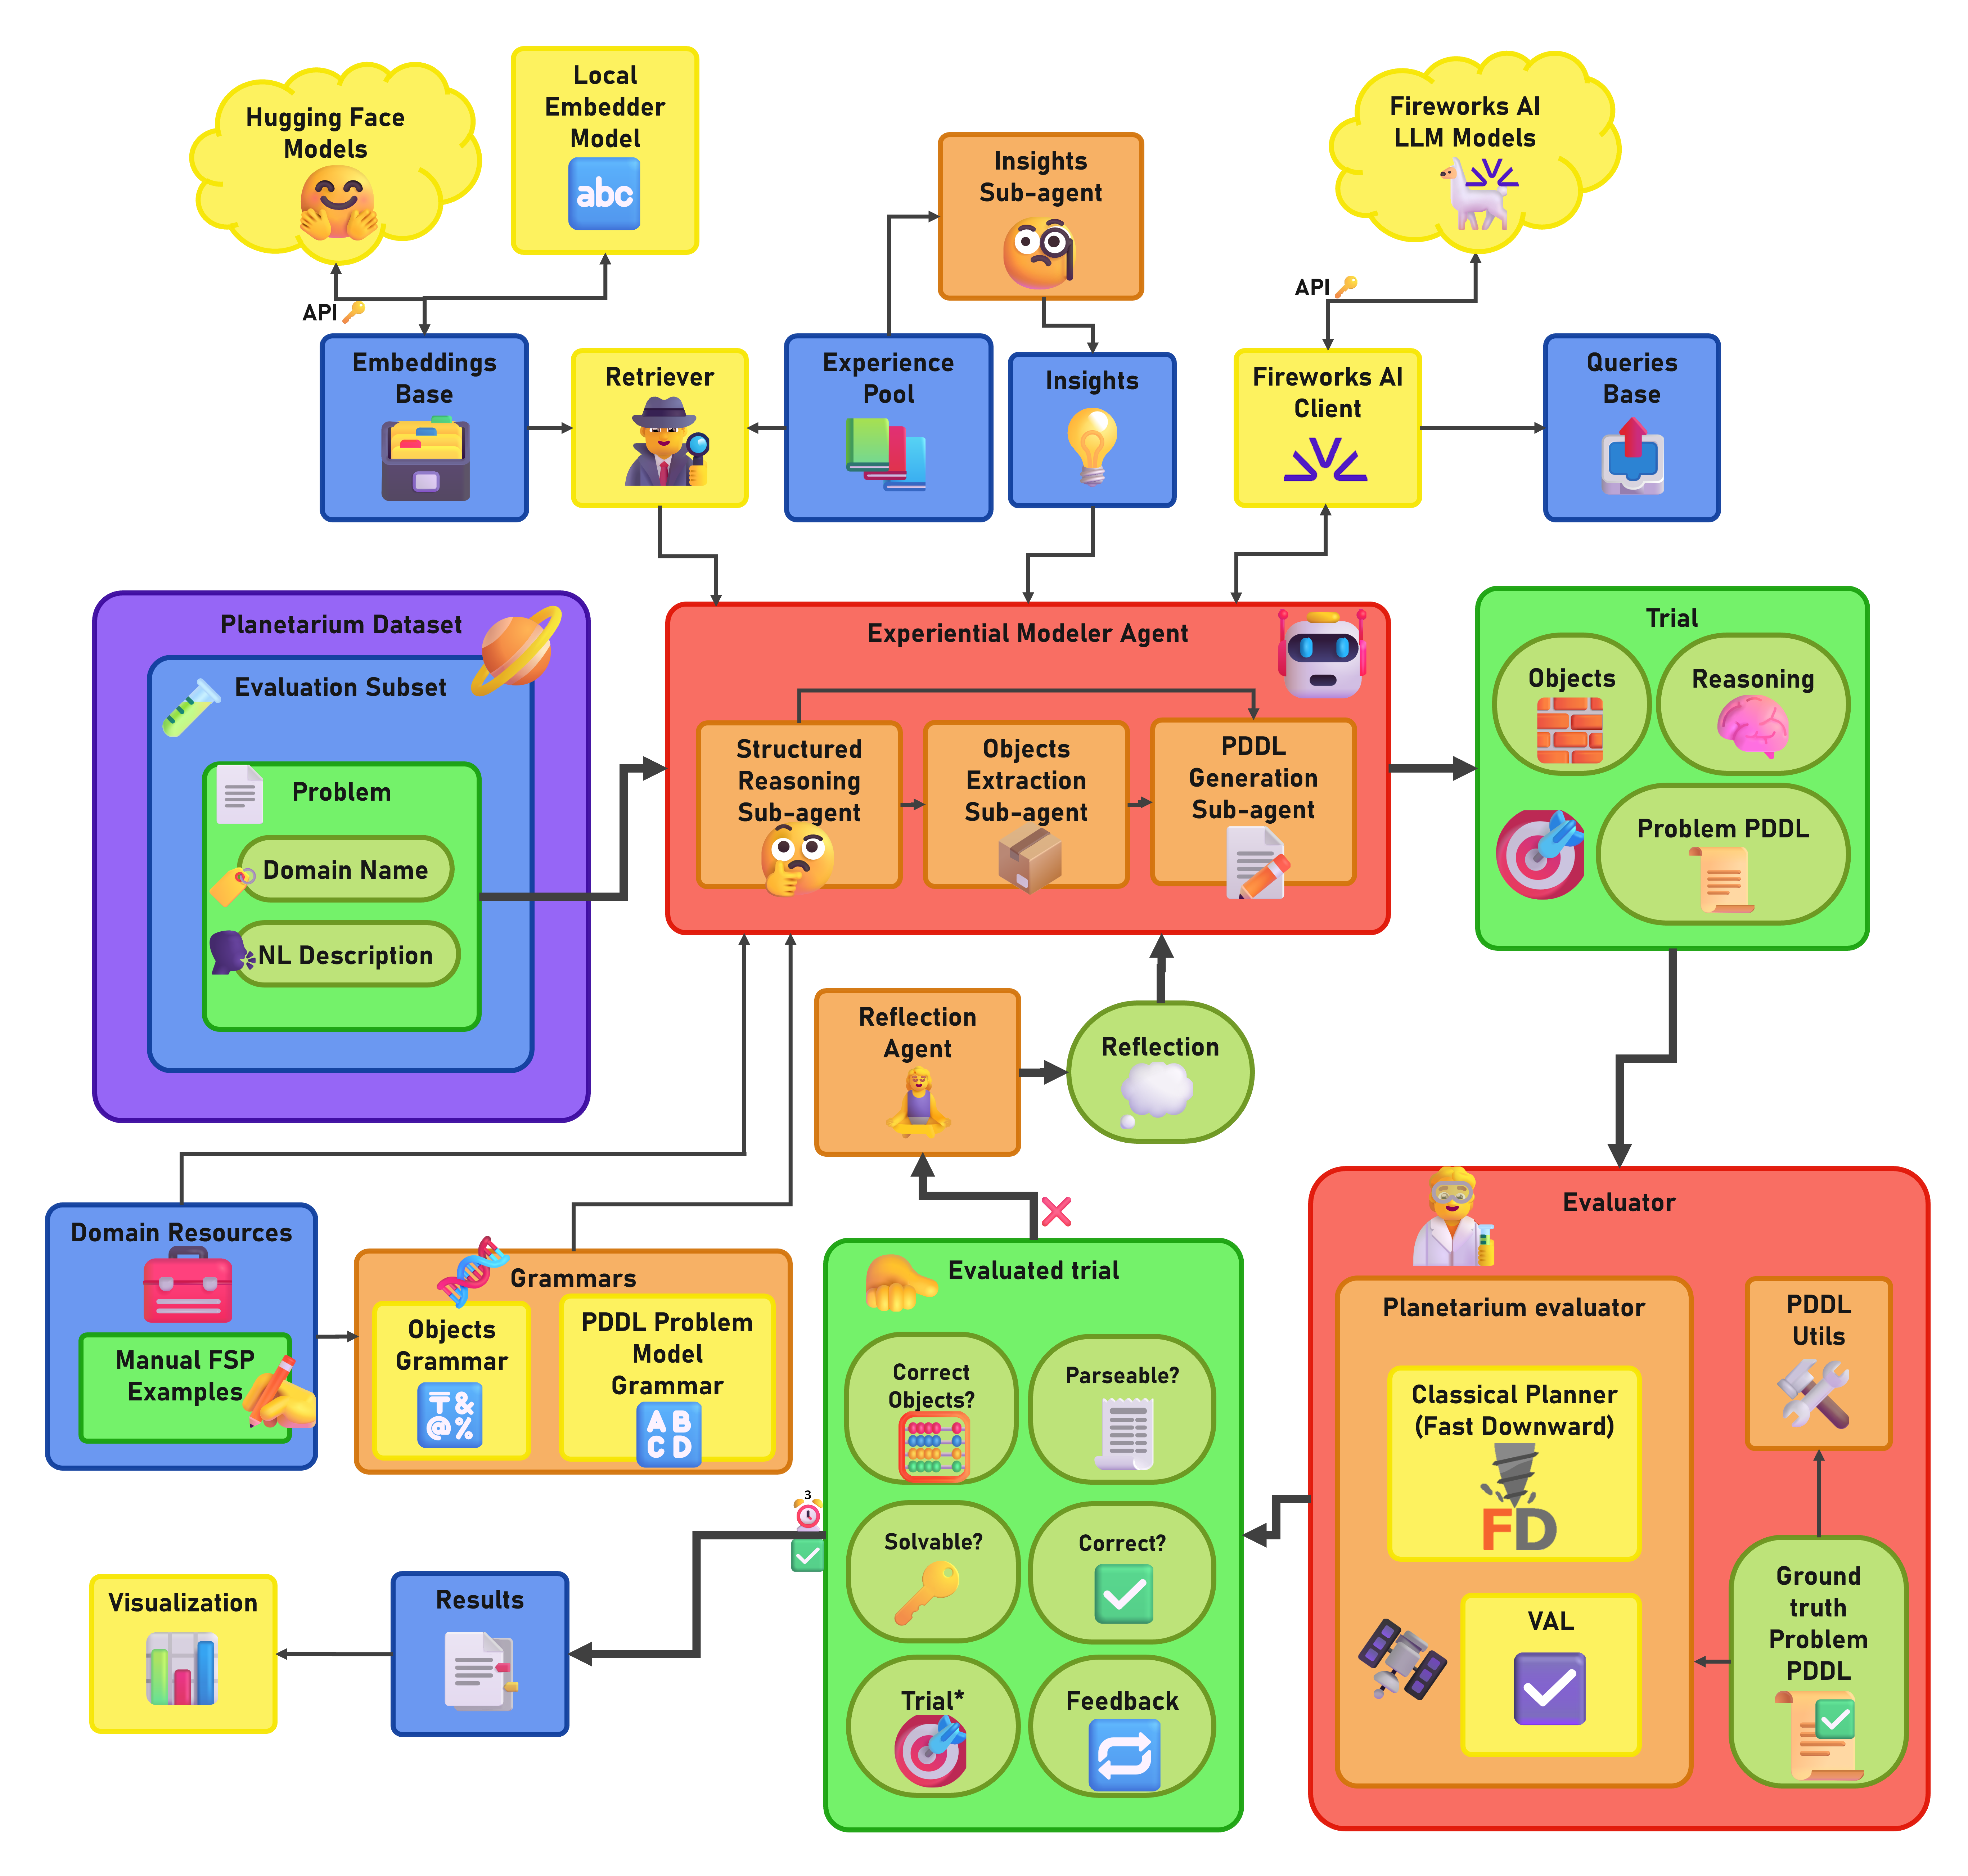
\includegraphics[width=0.9\textwidth]{Graphics/exp_evaluation.png}
\caption{Flujo de evaluación de los agentes modeladores experienciales propuestos.}
\label{fig:objects}
\end{figure}

\subsection{Reflexión}

Se propone un agente especializado en reflexionar sobre intentos fallidos de generación de modelos \textit{PDDL} de problemas de planificación. Su propósito es analizar los errores cometidos por un agente modelador al generar un modelo de problema, y proponer posibles correcciones a partir del análisis de retroalimentación proporcionado por la evaluación formal descrita en secciones anteriores.

Este agente de reflexión opera a partir de un \textit{prompt} cuidadosamente diseñado que sintetiza toda la información relevante del intento fallido, incluyendo la descripción del dominio, el modelo \textit{PDDL} del dominio, la descripción natural del problema, el razonamiento previo del agente modelador, los objetos utilizados, el modelo \textit{PDDL} generado en el intento fallido, y el \textit{feedback} obtenido tras la evaluación. Con base en esta información, el agente debe inferir la posible causa del fallo y sugerir modificaciones, de manera razonada y específica.

El \textit{prompt} instruye al modelo para que actúe como un agente experto en modelado que reflexiona sobre errores cometidos en la generación de problemas de planificación. Se le presenta un intento fallido de modelado junto con una descripción completa del contexto: dominio (nombre, explicación breve y modelo \textit{PDDL}), descripción natural del problema, razonamiento generado y objetos utilizados (si aplican), modelo generado y retroalimentación sobre el error. El agente debe considerar una jerarquía de posibles errores —errores sintácticos, problemas de solubilidad y errores semánticos— y entender que errores de menor nivel invalidan automáticamente la posibilidad de evaluar los de nivel superior (por ejemplo, un modelo con errores sintácticos no puede ser evaluado semánticamente)\footnote{Al menos bajo el alcance de esta tesis no es posible hacerlo de forma automática y determinista, pero sí sería posible que en un modelo con errores sintácticos un humano experto identifique el significado semántico subyacente y sus posibles errores.}.

El modelo debe generar un único párrafo en el que explique de forma razonada cuál pudo haber sido la causa del fallo, e indique explícitamente qué elementos deben ser corregidos: el estado inicial, el estado objetivo, o ambos. Esta reflexión se integra como una fase posterior al proceso de evaluación y puede ser utilizada por los agentes modeladores para fundamentar nuevos intentos. La capacidad de razonar sobre errores, explicarlos y proponer soluciones convierte a esta etapa en un componente crucial del ciclo iterativo de mejora basado en retroalimentación estructurada.

\section{Entrenamiento}

Con el objetivo de acumular conocimiento útil para abordar tareas futuras, se diseña un proceso de entrenamiento para el agente modelador experiencial. Este proceso consiste en dos fases bien diferenciadas: una fase de acumulación de experiencias y una fase de extracción de \textit{insights}.

La inspiración conceptual y metodológica para esta etapa proviene del trabajo presentado en \textit{ExpeL} \parencite{zhao2024expel}, el cual introdujo una estrategia sistemática de entrenamiento mediante intentos múltiples, autorreflexión y reutilización de trayectorias pasadas, tanto como ejemplos de \textit{FSP} como para la extracción de \textit{insights}.

En esta tesis se reutiliza y adapta dicho enfoque para el entrenamiento del agente modelador experiencial propuesto. Concretamente, se selecciona un subconjunto del \textit{dataset Planetarium} que tenga poca intersección con el subconjunto reservado para evaluación. Sobre este subconjunto se ejecuta un proceso iterativo, en el cual el agente intenta resolver cada una de las tareas de planificación como máximo tres veces, o hasta lograr una solución correcta.

Durante cada intento, el agente recibe como entrada la descripción natural del problema, el dominio \textit{PDDL} correspondiente, y un conjunto de ejemplos \textit{few-shot} fijos. En el primer intento, no se proporciona ninguna reflexión adicional. Sin embargo, si el intento falla, se activa el agente reflexionador descrito previamente, el cual genera una reflexión en lenguaje natural sobre las causas del fallo. Esta reflexión se incorpora al \textit{prompt} del siguiente intento, permitiendo al agente modelador considerar sus errores pasados y adaptar su estrategia en consecuencia. Este mecanismo de retroalimentación iterativa resulta clave para mejorar la tasa de éxito en intentos subsiguientes.

Todas las trayectorias generadas —ya sean fallidas o exitosas— son almacenadas en un \textit{Experience Pool} (repositorio de experiencias), que constituye una memoria a largo plazo del agente. Esta base de datos de experiencias tiene una doble función en el sistema. Por una parte, se utiliza como fuente para la recuperación de ejemplos exitosos mediante \textit{RAG} durante la fase de evaluación. Por otra, sirve como insumo para la fase de extracción de \textit{insights}, donde se analizan varias experiencias previas para identificar patrones útiles y generar recomendaciones generalizables. Esta segunda fase será detallada en la subsección siguiente.

Adicionalmente, se propone la incorporación de \textit{insights} agregados manualmente por expertos humanos, lo cual permite contrastar el conocimiento extraído automáticamente con el criterio experto, e incluso enriquecer el \textit{corpus} de recomendaciones disponibles durante la evaluación.

\begin{figure}[H]
\centering
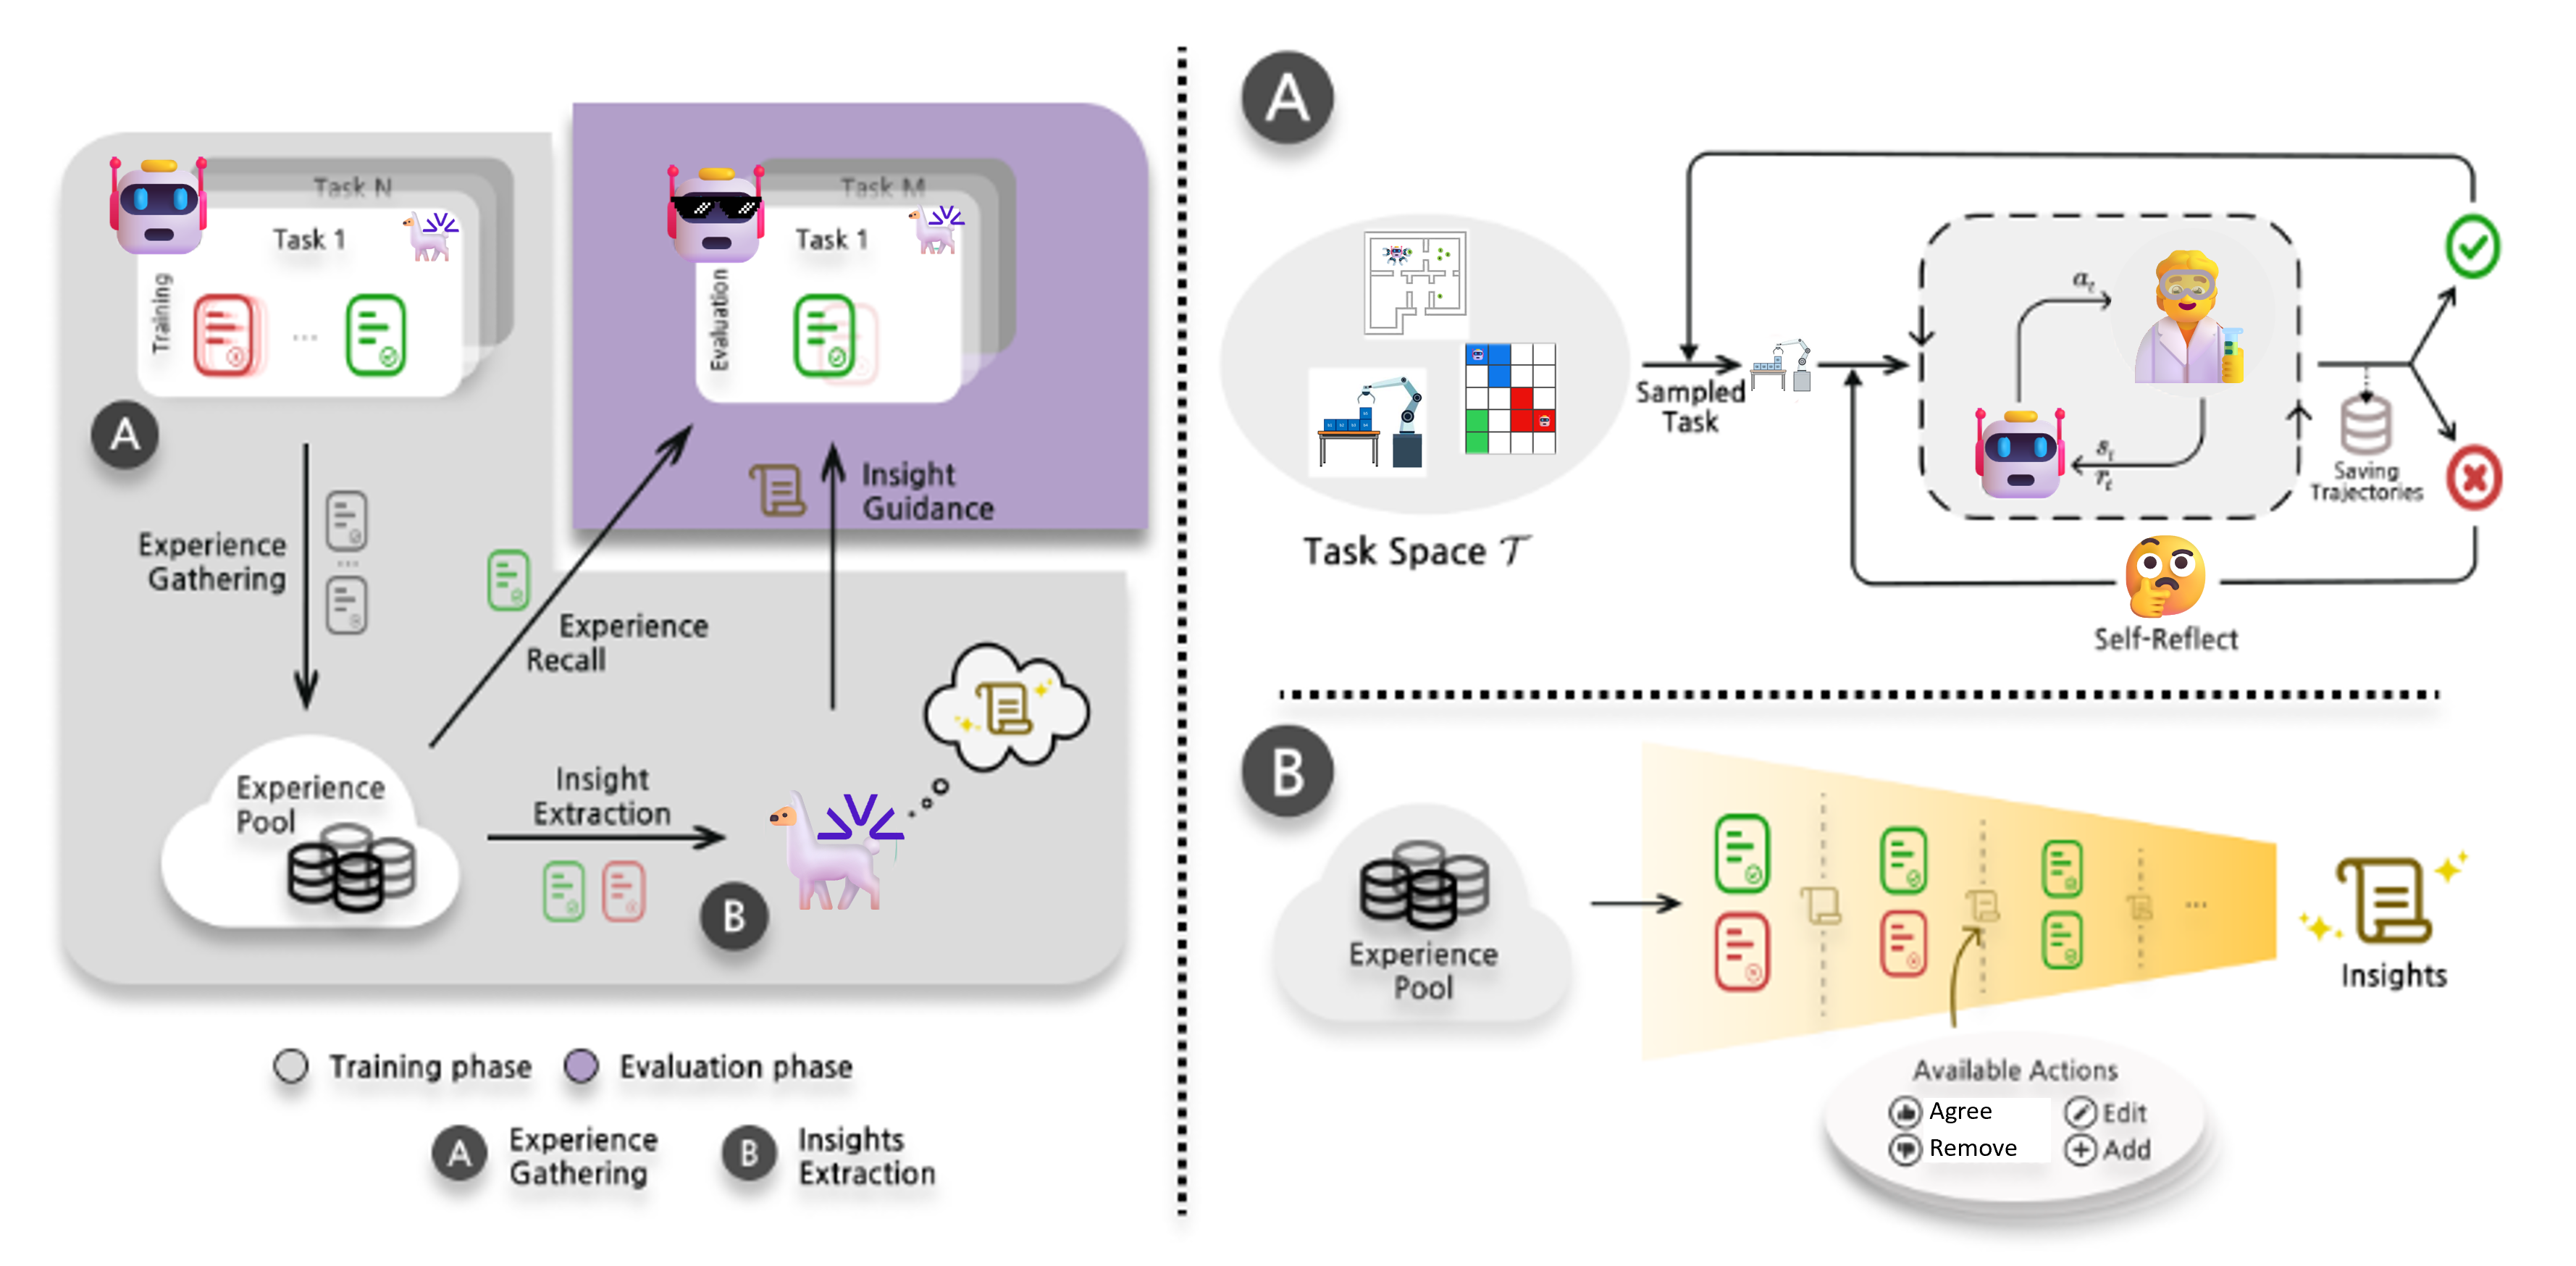
\includegraphics[width=0.9\textwidth]{Graphics/training.png}
\caption{Imagen adaptada del \textit{paper} de \textit{ExpeL} \parencite{zhao2024expel}. Izquierda: se opera en tres etapas: (1) Recolección de experiencias de éxito y fracaso en un \textit{pool}. (2) Extracción/abstracción de conocimiento entre tareas a partir de estas experiencias. (3) Aplicación de los conocimientos adquiridos y recuerdo de éxitos pasados en tareas de evaluación. Derecha: (A) Ilustra el proceso de recolección de experiencias a través del agente reflexionador, permitiendo reintentos de la tarea después de la autorreflexión sobre los fracasos. (B) Ilustra el paso de extracción de conocimiento. Cuando se le presentan pares de éxito/fracaso o una lista de $L$ éxitos, el agente modifica dinámicamente una lista existente de conocimientos $\hat{\iota}$ utilizando las operaciones \texttt{ADD}, \texttt{AGREE}, \texttt{REMOVE} y \texttt{EDIT}.}
\label{fig:training}
\end{figure}

A continuación se presenta el pseudocódigo que describe el proceso de entrenamiento:

\begin{algorithm}[H]
\caption{Entrenamiento del agente experiencial}
\label{alg:entrenamiento}
\SetKwInOut{Input}{Input}
\SetKwInOut{Output}{Output}

\Input{\\
\hspace{1em} Agente modelador \(\mathcal{A}_{\mathrm{mod}}\) \\
\hspace{1em} Conjunto de tareas de entrenamiento \(\mathcal{T}_{\mathrm{train}}\) \\
\hspace{1em} Número máximo de intentos por tarea \(Z\) \\
\hspace{1em} Indicador de continuación de entrenamiento previo: \texttt{resume} \\
\hspace{1em} Indicador de retroalimentación humana: \texttt{human\_feedback}
}
\Output{\\
\hspace{1em} Conjunto acumulado de experiencias \(B\)
}

Inicializar ruta de progreso y cargar o reiniciar estado\;
Inicializar conjunto de experiencias: \(B \leftarrow \emptyset\)\;

\eIf{\texttt{resume}}{
    Cargar índice de tarea \(i\) desde archivo de progreso\;
}{
    \(i \leftarrow 0\)\;
    Guardar progreso inicial en disco\;
}

\For{\(i = i\) \KwTo \(|\mathcal{T}_{\mathrm{train}}|-1\)}{
    \(t_i \leftarrow \mathcal{T}_{\mathrm{train}}[i]\)\;
    Inicializar reflexiones previas: \(\lambda \leftarrow \emptyset\)\;

    Llamar \(\mathcal{A}_{\mathrm{mod}}.\texttt{asignar\_tarea}(t_i)\)\;

    \For{\(z = 0\) \KwTo \(Z-1\)}{
        Resolver tarea: \(\mathcal{P}_{\pi}^{(z)} \leftarrow \mathcal{A}_{\mathrm{mod}}.\texttt{resolver}()\)\;

        Evaluar resultado: \(e_{i,z} \leftarrow \texttt{evaluar}(t_i, \mathcal{P}_{\pi}^{(z)})\)\;

        Guardar experiencia:
        \(
        B \leftarrow B \cup \texttt{store\_exp}(t_i,\ z,\ \lambda[z-1],\ \mathcal{P}_{\pi}^{(z)},\ e_{i,z})
        \)

        \eIf{\(e_{i,z}.\texttt{correct} = \texttt{True}\)}{
            \textbf{break}\;
        }{
            \eIf{\(z = Z-1\) \textbf{y} \texttt{human\_feedback}}{
                Mostrar evaluación fallida y solicitar entrada humana\;
                \(\nu_z \leftarrow \texttt{input()} \)\;
            }{
                Generar reflexión automática:
                \(
                \nu_z \leftarrow \texttt{reflect}(\mathcal{A}_{\mathrm{mod}}.P_{\mathrm{desc}},\ \mathcal{A}_{\mathrm{mod}}.D,\ \lambda,\ \mathcal{P}_{\pi}^{(z)},\ e_{i,z})
                \)
            }
            Agregar reflexión: \(\lambda \leftarrow \lambda \cup \{\nu_z\}\)\;
            Actualizar \(\mathcal{A}_{\mathrm{mod}}.\tau \leftarrow \mathcal{A}_{\mathrm{mod}}.\tau \cup (\mathcal{P}_{\pi}^{(z)},\ e_{i,z},\ \nu_z)\)\;
        }
    }
    Insertar \(B\) en base persistente\;
    Actualizar archivo de progreso con índice \(i\)\;
}
Marcar entrenamiento como completado en archivo de progreso\;

\Return \(B\)\;
\end{algorithm}

\subsection{Fase de extracción de \textit{insights}}

Una vez concluida la fase de acumulación de experiencias, se procede a una segunda fase centrada en la generación y depuración de \textit{insights}, con el propósito de sintetizar lecciones aprendidas a partir de las trayectorias recopiladas. Esta fase busca abstraer conocimientos útiles tanto específicos del dominio como generales, que puedan ser aprovechados por el agente modelador durante la evaluación para mejorar su desempeño.

En esta tesis se retoma la propuesta metodológica presentada en \textit{ExpeL} \parencite{zhao2024expel}, donde se argumenta que un agente puede analizar sus experiencias de manera sistemática para extraer conocimiento valioso. En particular, se identificaron dos mecanismos complementarios de análisis. El primero consiste en comparar una trayectoria fallida con una trayectoria exitosa sobre la misma tarea, lo cual permite identificar de forma concreta las acciones incorrectas en contraste con las correctas. El segundo mecanismo se basa en el análisis de patrones comunes entre múltiples trayectorias exitosas, provenientes de distintas tareas dentro de un mismo dominio. Esta segunda forma de análisis permite detectar buenas prácticas recurrentes, que pueden ser generalizadas como reglas efectivas de modelación.

Tomando como base dicha propuesta, se estructura la fase de extracción de \textit{insights} en dos modos operativos principales:

\begin{itemize}
  \item \textbf{Comparación entre intentos fallidos y exitosos del mismo problema.} Para cada problema del conjunto de entrenamiento resuelto con éxito, se identifican todos los intentos fallidos previos al exitoso realizados por el agente. Con estos datos se construyen pares de la forma $(\textit{incorrecto}_i, \textit{correcto})$, donde cada $\textit{incorrecto}_i$ representa una trayectoria fallida del mismo problema, y $\textit{correcto}$ corresponde a la solución exitosa. Estos pares permiten al sistema inferir causas de error específicas, reconocer desviaciones de comportamientos correctos y extraer recomendaciones de mejora concretas.
  
  \item \textbf{Comparación de múltiples soluciones correctas dentro de un mismo dominio.} Para cada dominio de planificación, se coleccionan todas las trayectorias exitosas generadas durante la fase anterior. Estas soluciones se agrupan en lotes (\textit{batches}) de tamaño configurable; en este trabajo se emplean \textit{batches} de tamaño 2. Estos lotes son utilizados para identificar patrones comunes entre problemas diferentes pero enmarcados en un mismo contexto semántico. De esta forma, se buscan regularidades y estructuras repetidas que reflejen buenas prácticas aplicables a otros problemas del dominio.
\end{itemize}

El sistema responsable de esta fase —denominado Agente de \textit{Insights}— recibe como entrada ambos conjuntos: los pares $(\textit{incorrecto}_i, \textit{correcto})$ y los \textit{batches} de trayectorias exitosas. A partir de ellos, es capaz de actualizar progresivamente su base interna de \textit{insights}, acumulando información que luego podría emplearse para guiar al agente modelador durante la evaluación.

Los \textit{insights} extraídos se clasifican en tres categorías distintas:

\begin{itemize}
  \item \textbf{Conocimiento del mundo:} Incluye información semántica específica sobre el dominio, como el significado y uso típico de predicados, restricciones físicas o abstractas implícitas, y relaciones relevantes entre objetos. Este tipo de conocimiento permite al agente comprender mejor la estructura lógica subyacente al dominio de planificación.

  \item \textbf{Reglas para la planificación en el dominio:} Contiene estrategias específicas de modelación aprendidas por observación. Por ejemplo, el uso correcto de ciertos predicados en la formulación de problemas, la inclusión necesaria de ciertos objetos o acciones, o la estructuración típica de los objetivos en ese dominio.

  \item \textbf{Reglas generales de modelación:} Se refiere a principios que resultan útiles en múltiples dominios, y que no dependen de un contexto semántico específico. Estos incluyen, por ejemplo, recomendaciones sobre la forma de declarar objetos, cómo seleccionar hechos iniciales relevantes, o patrones efectivos en la formulación de metas.
\end{itemize}

La base de \textit{insights} se inicializa vacía, y es construida de forma incremental a medida que se procesan los conjuntos de experiencias mencionados. El agente de extracción evalúa la utilidad y relevancia de cada observación, descartando aquellas poco informativas o irrelevantes, y consolidando las más consistentes o frecuentes. Esta base se diseña como un componente reutilizable, que puede enriquecer progresivamente su contenido con nuevas experiencias de entrenamiento o intervención humana experta.

Este mecanismo de análisis diferenciado de errores y éxitos, junto con la categorización estructurada del conocimiento, permite dotar al sistema de una memoria inferencial rica, orientada a facilitar la generalización y la transferencia de aprendizajes durante la fase de evaluación.

\section{Agente de \textit{Insights}}

Como se explicó en la sección anterior, los \textit{insights} representan unidades de conocimiento estructurado, útiles para la modelación de problemas de planificación automática. Cada \textit{insight}, independientemente de su tipo (conocimiento del mundo, reglas del dominio o reglas generales), se representa mediante una breve descripción textual y un valor numérico que indica su relevancia acumulada, interpretado como una medida de confianza, utilidad o frecuencia.

Con el objetivo de mantener y actualizar este conjunto de \textit{insights}, se propone un sistema especializado: el \textit{Agente de Insights}. Este agente opera sobre la base de un conjunto de acciones bien definidas que le permiten construir, refinar y filtrar progresivamente el conocimiento extraído de las experiencias almacenadas.

Este enfoque toma como referencia directa el mecanismo descrito por \textit{ExpeL} \parencite{zhao2024expel}, donde se propone iniciar con un conjunto vacío de \textit{insights}, y actualizarlo de forma iterativa a partir del análisis de pares $(\textit{fallo}, \textit{éxito})$ o listas de trayectorias exitosas, previamente recolectadas en la fase de acumulación de experiencias. En cada iteración, el modelo de lenguaje recibe alguno de estos conjuntos como contexto, y debe decidir qué operaciones aplicar sobre los \textit{insights} actuales.

Las operaciones permitidas por el agente son las siguientes:

\begin{itemize}
  \item \textbf{ADD} (agregar): introduce un nuevo \textit{insight} que no esté representado aún en la base. Este nuevo \textit{insight} es añadido con el texto sugerido por el agente, y un valor inicial de relevancia igual a 2. Esta operación permite extender el conocimiento acumulado.

  \item \textbf{EDIT} (editar): modifica el contenido textual de un \textit{insight} ya existente, con el objetivo de mejorar su claridad, generalidad o aplicabilidad. Esta operación también incrementa su valor numérico en 1, como señal de reafirmación de su utilidad tras la edición.

  \item \textbf{AGREE} (confirmar): reafirma la validez de un \textit{insight} existente, confirmando que sigue siendo relevante para los ejemplos analizados. Esta operación incrementa su valor numérico en 1.

  \item \textbf{REMOVE} (eliminar o devaluar): indica desacuerdo con un \textit{insight} actual, por considerarlo erróneo, irrelevante, redundante, demasiado específico, o \textit{superseded} (superado por otro más general o actualizado). Esta operación disminuye su valor numérico. Para controlar la sobreacumulación de \textit{insights}, se define un umbral $M$ (establecido en 10). Si el número de \textit{insights} de un tipo dado es mayor o igual a $M$, esta operación disminuye el valor numérico del \textit{insight} seleccionado en 3 unidades; en caso contrario, la disminución es de 1. Si el valor resultante no es positivo, el \textit{insight} es eliminado de la base.
\end{itemize}

Esta política de actualización se diseña para ser robusta frente a sesgos o errores puntuales en las trayectorias, permitiendo reforzar progresivamente aquellos \textit{insights} que son validados de forma reiterada en contextos distintos, y depurar los que no resultan útiles o se contradicen con ejemplos posteriores. Este diseño también considera que incluso trayectorias exitosas pueden ser subóptimas, y por tanto sus recomendaciones deben ser sometidas a verificación iterativa.

Además, para mantener la estabilidad y eficiencia del sistema, se establece un número máximo de operaciones por tipo de \textit{insight} durante cada sesión de procesamiento. En este trabajo, se fija un límite de 4 operaciones por tipo, lo cual obliga al agente a priorizar sus modificaciones más relevantes en cada interacción.

Mediante este mecanismo, se pretende que el \textit{Agente de Insights} construya de manera incremental una base de conocimientos estructurados y validados, capaz de asistir al agente modelador durante la etapa de evaluación, tanto en la selección de hechos iniciales como en la formulación de objetivos o en la verificación de consistencia semántica.

Para permitir que el agente opere sobre conjuntos complejos y estructurados de conocimiento, se concibe un \textit{prompt} parametrizable y flexible que guía el comportamiento del modelo de lenguaje durante la fase de generación o depuración de \textit{insights}. Este \textit{prompt} adopta una estructura instruccional clara, definiendo el contexto del dominio, las reglas operacionales, las limitaciones por tipo de \textit{insight}, y la información sobre los intentos previos que deben ser tenidos en cuenta.

Al igual que en agentes anteriores, algunos componentes del prompt son completados dinámicamente en función del dominio en cuestión, del estado actual de la base de \textit{insights} y de las experiencias a analizar. El nombre del dominio, su descripción breve en lenguaje natural y su correspondiente modelo en \textit{PDDL} se extraen directamente de la base de datos del dominio, y constituyen el contexto sobre el que se espera que el agente razone. Junto a ello, se incluye el conjunto actual de \textit{insights} organizados en las tres categorías establecidas (conocimiento del mundo, reglas específicas del dominio y reglas generales), presentados de forma numerada para su referencia.

El \textit{prompt} también informa al agente sobre el límite máximo de operaciones por tipo de \textit{insight}, y define de forma explícita los elementos que debe considerar al tomar decisiones, como reflexiones, retroalimentaciones de evaluación, o trayectorias exitosas y/o fallidas previas. Según el procedimiento que haya generado ese conjunto de entrada, se incorpora también una descripción del modo de extracción, y si se detecta una cantidad excesiva de \textit{insights} de cierto tipo (es decir, si se ha superado un umbral establecido), se añade una instrucción adicional que obliga al agente a priorizar operaciones de depuración o eliminación, en lugar de seguir incrementando la base de conocimiento.

Este \textit{prompt} es utilizado durante la fase de construcción del conocimiento derivado, permitiendo al agente analizar críticamente los datos acumulados y refinar su base de \textit{insights} de manera progresiva, controlada y fundamentada.

\subsubsection{Comparación de un par de intentos de un mismo problema, uno fallido y uno exitoso}

Uno de los mecanismos de extracción de \textit{insights} es la comparación directa entre un intento fallido y uno exitoso sobre el mismo problema. Este enfoque permite al agente identificar cambios clave que condujeron a una solución correcta, extrayendo lecciones reutilizables que pueden informar futuros intentos. Esta estrategia se inspira directamente en el enfoque de \textit{ExpeL}, donde se formaliza la reflexión comparativa como una técnica eficaz para detectar errores frecuentes, sistematizar buenas prácticas y fortalecer el desempeño del agente a lo largo del tiempo.

En este modo de operación, el \textit{prompt} proporcionado al agente incluye información detallada sobre ambos intentos. Para definir el contexto, se especifica que se trata de dos intentos —uno exitoso y otro fallido— de una misma tarea de planificación, en los cuales el agente modelador recibió siempre la misma descripción del dominio, el archivo \textit{PDDL} del dominio, y una descripción en lenguaje natural del problema. Esta información contextual se incluye con una redacción explícita que enmarca la tarea de contraste.

Luego, se le indica al modelo que debe enfocar su análisis en patrones, errores recurrentes o lecciones que puedan deducirse al comparar ambos intentos. El bloque posterior incluye una representación completa del intento fallido —con razonamiento y objetos seleccionados (si aplican), el modelo \textit{PDDL} generado y la retroalimentación obtenida— así como la reflexión generada tras la evaluación si esta se encuentra disponible. A continuación, se presenta también el intento exitoso con su salida generada, lo que permite una visión paralela de las decisiones tomadas antes y después de corregir los errores. Esta estructura está pensada para proporcionar un marco claro al agente, en el que puede detectar, comparar y abstraer conocimiento útil a partir de los contrastes observados.

\subsubsection{Comparación de varias soluciones correctas de distintos problemas del mismo dominio}

Además del anterior, se incorpora un modo de extracción que opera sobre múltiples intentos exitosos correspondientes a distintos problemas del mismo dominio. Este enfoque busca generalizar buenas prácticas a partir de trayectorias que han demostrado ser válidas, capturando regularidades que puedan aplicarse a nuevas instancias similares. De nuevo, este procedimiento sigue las recomendaciones de \textit{ExpeL}, donde se argumenta que las soluciones correctas también son fuentes valiosas de conocimiento estructurado.

En este caso, el \textit{prompt} indica explícitamente que todas las entradas corresponden a intentos exitosos en un mismo dominio, manteniendo el contexto —la descripción del dominio y su modelo en \textit{PDDL}— solo variando la formulación del problema en lenguaje natural, para cada tarea analizada. Esta información se incorpora consecutivamente, y prepara al agente para analizar los datos bajo un criterio común.

El conjunto de datos presentado al agente incluye varios intentos exitosos, cada uno estructurado de forma consistente, con información sobre el problema, el razonamiento realizado y los objetos determinados (si aplican), y el modelo generado. Una instrucción dada orienta al modelo a identificar patrones o lecciones presentes en estas soluciones válidas, permitiéndole extraer \textit{insights} que refuercen estrategias útiles y recurrentes dentro del mismo dominio de planificación.

\section{RAG}

Durante la fase de acumulación de experiencias, se generan múltiples soluciones correctas de modelación de problemas de planificación. Estas soluciones exitosas se estiman útiles como ejemplos de \textit{FSP} para resolver nuevos problemas, mediante \textit{RAG}.

Cuando se presenta una nueva tarea a resolver, y se requieren $k$ ejemplos de \textit{FSP}, el sistema selecciona las $k$ soluciones almacenadas en el \textit{Experience Pool} cuya descripción en lenguaje natural sea más similar a la del nuevo problema. Esta similitud se determina mediante el cálculo de \textit{embeddings} de lenguaje natural de las descripciones de los problemas, y el uso de la medida de \textit{cosine similarity} (similitud del coseno) para obtener las más cercanas.

En el capítulo de Implementación se analiza a detalle el proceso que se lleva a cabo.